%% LyX 2.3.2 created this file.  For more info, see http://www.lyx.org/.
%% Do not edit unless you really know what you are doing.
\documentclass{article}
\usepackage[utf8]{inputenc}
\usepackage{geometry}
\geometry{verbose,tmargin=2.5cm,bmargin=2cm,lmargin=2cm,rmargin=2cm}
\usepackage{array}
\usepackage{verbatim}
\usepackage{float}
\usepackage{units}
\usepackage{mathtools}
\usepackage{amsmath}
\usepackage{graphicx}

\makeatletter

%%%%%%%%%%%%%%%%%%%%%%%%%%%%%% LyX specific LaTeX commands.
%% Because html converters don't know tabularnewline
\providecommand{\tabularnewline}{\\}

%%%%%%%%%%%%%%%%%%%%%%%%%%%%%% Textclass specific LaTeX commands.
\newcommand{\lyxaddress}[1]{
	\par {\raggedright #1
	\vspace{1.4em}
	\noindent\par}
}

%%%%%%%%%%%%%%%%%%%%%%%%%%%%%% User specified LaTeX commands.
\usepackage{xr}
\externaldocument{Paper_req-550_V1.0.2}
\usepackage{lineno}
\usepackage{xcolor}
\usepackage{tikz}
\usetikzlibrary{arrows}

\newcommand{\bs}[1]{\boldsymbol{#1}}
\newcommand{\add}[1]{\textcolor{red}{#1}}
\newcommand{\oran}{\mathrm{o}}
\newcommand{\g}{\mathrm{g}}
\newcommand{\X}{\mathrm{X}}
\newcommand{\Y}{\mathrm{Y}}
\newcommand{\PP}{\mathrm{P}}
\newcommand{\EE}{\mathrm{E}}
\newcommand{\RR}{\mathrm{RR}}
\newcommand{\DD}{\mathrm{DD}}

\newcommand{\HH}{\mathrm{H}}
\newcommand{\A}{\mathrm{A}}
\newcommand{\I}{\mathrm{I}}
\newcommand{\M}{\mathrm{M}}
\newcommand{\OO}{\mathrm{O}}

\newcommand{\sh}{\mathrm{sh}}
\newcommand{\nullm}{\mathrm{null}}
\newcommand{\intv}{\mathrm{intv}}
\newcommand{\family}{\mathrm{visit}}
\newcommand{\care}{\mathrm{care}}
\newcommand{\Exp}{\mathrm{exp}}
\newcommand{\onset}{\mathrm{onset}}

\makeatother

\begin{document}
\title{Supplementary Methods and Results\\Empowering the crowd: Feasible
strategies \\ to minimize the spread of COVID-19 \\ in informal
settlements}
\author{Alberto Pascual-García$^{(1,*)}$, Jordan Klein$^{(2)}$, Jennifer
Villers$^{(3,\land)}$, \\ Eduard Campillo-Funollet$^{(4,\wedge)}$,
Chamsy Sarkis$^{(5)}$}

\maketitle
\medskip{}


\lyxaddress{\begin{center}
(1) Institute of Integrative Biology. ETH-Zürich. Zürich, Switzerland.
\\ (2) Office of Population Research. Princeton University. Princeton,
NJ, USA. \\ (3) Princeton Environmental Institute. Princeton University.
Princeton, NJ, USA. \\ (4) Genome Damage and Stability Centre. University
of Sussex. Brighton, United Kingdom. \\ (5) Pax Syriana Foundation.
Valetta, Malta. \\ ($\land$) Equal contribution. \\ ({*}) correspondence:
alberto.pascual@env.ethz.ch
\par\end{center}}

\newpage{}

\section{Parameterization of the model}

\subsection{Derivation of fixed parameters (Table \ref{tab:FixedParams} in Main
Text)}

To estimate the latent period ($\nicefrac{1}{\delta_{\EE}}$), we
calculated the difference between randomly generated incubation ($\nicefrac{1}{\delta_{\EE}}+\nicefrac{1}{\delta_{\PP}}$)
and presymptomatic ($\nicefrac{1}{\delta_{\PP}}$) periods. We estimated
the presymptomatic period using results reported by He et al. \cite{he2020temporal}
and found they best fit a Gompertz distribution with a mean of 2.3
days (95\% CI: 0.8-3.0). Since a correction of these by Ashcroft et
al. \cite{ashcroft_covid-19_2020} suggests they significantly underestimate
the presymptomatic period's upper bound, we estimated that the true
presymptomatic period follows a Gaussian distribution around the mean
(95\% CI: 0.8-3.8). However, this presymptomatic period distribution
implies a non-negligible probability of a negative latent period.
To correct this discrepancy, we assumed a minimum latent period of
.5 days \cite{harcourt2020severe}. Time from symptom onset to death
in critical cases ($\nicefrac{1}{\alpha}$) is estimated using time
from symptom onset to ICU admission in Wang et al \cite{wang2020clinical}.

\subsection{Population structure of demographic-classes derivation (Table \ref{tab:PopParams}
in Main Text)}

In April, 2020, 40.7\% of the population in informal IDP camps in
Northern Syria was aged 0-12, 53.4\% aged 13-50, and 5.9\% aged 51+
\cite{noauthor_syrian_nodate}. To estimate the proportion of each
age group with comorbidities, we calculated the weighted average age-specific
comorbidity prevalence of the 4 most common comorbidities in the Syrian
refugee populations in Jordan and Lebanon: hypertension, cardiovascular
disease, diabetes, and chronic respiratory disease \cite{doocy_prevalence_2015,doocy_prevalence_2016}.
We standardized these weighted averages to the age structure of IDPs
in Northern Syria and estimated that 11.7\% of people aged 13-50 have
comorbidities, while 62.9\% of people aged 51+ have comorbidities.

\subsection{Derivation of transmissibility parameters}

The probability of infection if there is a contact between a susceptible
and an infected person depends on the stage of the disease, denoted
$\tau\beta_{\PP}$, $\tau\beta_{\A}$, $\tau\beta_{\I}$ or $\tau\beta_{\HH}$
depending upon whether the infected individual is in the presymptomatic
($P_{i}$), symptomatic ($I_{i}$), asymptomatic ($A_{i}$), or hospitalized
compartment ($H_{i}$), respectively. We estimated these parameters
in two steps. In the following section, we estimate the $\beta_{\X}$
parameters ($\X\in\{\PP,\A,\I,\HH\}$) which represent the relative
transmissibility of each stage with respect to the maximum transmissibility
$\tau$. After this calculation, we present our estimate for the maximum
transmissibility parameter $\tau$.

\subsubsection*{Relative transmissibilities $\beta$ (Table \ref{tab:FixedParams}
in Main Text)}

We start by considering the transmissibility of the presymptomatic
stage for those individuals becoming symptomaticas a reference ($\beta_{\PP\rightarrow\I}=1)$,
since the probability of infection from contact with an individual
at this epidemiological stage is highest \cite{he_temporal_2020}.
Next, we set the contribution of each epidemiological stage to infectivity
as proportional to $\beta_{\X}/\gamma_{\X}$, with $1/\gamma_{\X}$
the duration of stage $\X$. Following He et al, we estimate the proportion
of infectivity that occurs at the presymptomatic stage ($\X\in\{\PP\}$)
as the area under the infectivity curve prior to symptom onset, $AUC_{\PP}$,
and the proportion of infectivity that occurs at symptomatic stages
($\X\in\{\I,\HH\}$) as the area under the infectivity curve after
symptom onset, $1-AUC_{\PP}$ \cite{he_temporal_2020}:

\begin{equation}
\frac{AUC_{\PP}}{(1-AUC_{\PP})}\approx\frac{\frac{\beta_{\PP\rightarrow\I}}{\delta_{\PP}}}{\frac{\beta_{\I}}{\gamma_{\I}}+\frac{\beta_{\HH}}{\gamma_{\HH}}}\label{eq:AUC_P}
\end{equation}

We then considered the quantity $\rho_{\HH\I}$, the ratio of the
viral culture positive test rate in hospitalized patients 7-16 days
since start of symptoms to the positive test rate in patients 0-6
days since start of symptoms from van Kampen et al.\cite{van_kampen_shedding_2020}.
Similarly, the relative risk of asymptomatic transmission to symptomatic
transmission according to Byambasuren et al. is expressed as $\rho_{\A\I}$
\cite{byambasuren_estimating_2020}:

\begin{equation}
\beta_{\A}=\beta_{\I}\rho_{\A\I}
\end{equation}

\begin{equation}
\beta_{\HH}=\beta_{\I}\rho_{\HH\I}
\end{equation}

Considering these relationships we rewrite Eq. \ref{eq:AUC_P} to
obtain the desired parameters:

\begin{equation}
\beta_{\I}=\frac{\beta_{\PP\rightarrow\I}\gamma_{\I}\gamma_{\HH}(1-AUC_{\PP})}{AUC_{\PP}\delta_{\PP}(\gamma_{\HH}+\rho_{\HH\I}\gamma_{\I})}
\end{equation}

\begin{equation}
\beta_{\A}=\frac{\rho_{\A\I}\beta_{\PP\rightarrow\I}\gamma_{\I}\gamma_{\HH}(1-AUC_{\PP})}{AUC_{\PP}\delta_{\PP}(\gamma_{\HH}+\rho_{\HH\I}\gamma_{\I})}
\end{equation}

\begin{equation}
\beta_{\HH}=\frac{\rho_{\HH\I}\beta_{\PP\rightarrow\I}\gamma_{\I}\gamma_{\HH}(1-AUC_{\PP})}{AUC_{\PP}\delta_{\PP}(\gamma_{\HH}+\rho_{\HH\I}\gamma_{\I})}.
\end{equation}

The values of $AUC_{\PP}$, $\rho_{\A\I}$ and $\rho_{\HH\I}$ are
presented in Table \ref{tab:TransParams}, and the values of $\beta_{\X}$
in Main Text. Since the derivation was made relative to presymptomatic
individuals that will become presymptomatic, we should also estimate
the transmissibility of all presymptomatic individuals ($\beta_{\PP}$),
i.e. also including those that will be asymptomatic. Since the proportion
of presymptomatic that will become symptomatic is known (encoded in
$f$ in Eqs. \ref{eq:System1}--\ref{eq:System8} in Main Text) we
considered that the relative transmissibility between presymptomatic
individuals becoming symptomatic, and those becoming asymptomatic,
is the same than between symptomatic and asymptomatic individuals
($\rho_{\A\I}$). Following these considerations, the total transmissibility
is computed as:

\[
\beta_{\P}=f\beta_{\PP\rightarrow\I}+(1-f)\rho_{\A\I}\beta_{\PP\rightarrow\I}.
\]

\begin{table}[h]
\begin{tabular}{|>{\centering}m{0.1\textwidth}|>{\centering}m{0.275\textwidth}|>{\centering}m{0.275\textwidth}|>{\centering}m{0.1\textwidth}|>{\centering}m{0.1\textwidth}|}
\hline 
Parameter & Description & Value & Distribution & Reference\tabularnewline
\hline 
\hline 
$AUC_{\PP}$ & Presymptomatic area under infectivity curve & 0.44 (95\% CI: .30-.57) & Gaussian & \cite{he_temporal_2020}\tabularnewline
\hline 
$\rho_{\A\I}$ & Ratio of asymptomatic to symptomatic infectiousness & 0.58 (95\% CI: .34-.99) & Lognormal & \cite{byambasuren_estimating_2020}\tabularnewline
\hline 
$\rho_{\HH\I}$ & Ratio of hospitalized to symptomatic infectiousness & 0.48 & \_ & \cite{van_kampen_shedding_2020}\nocite{he_temporal_2020}\tabularnewline
\hline 
\end{tabular}

\caption{\label{tab:TransParams}\textbf{Relative transmissibility parameters.}}
\end{table}


\subsubsection*{Maximum transmissibility parameter $\tau$}

\begin{comment}
The derivation of R0 for a SIR type model following description of
'Mathematical Tools for Understanding Infectious Disease Dynamics'
written by Odo Diekmann, Hans Heesterbeek and Tom Britton. See chapter
7, section 2 'Next-generation matrix for compartmental systems'.
\end{comment}
{} %
\begin{comment}
1) Define the infected subsystem, i.e. all equations that include
compartments where individuals can get infected. 2) Linearize the
subsystem in the disease-free equilibrium. 3) Find the next generation
matrix (NGM) with large domain ($K_{L}$) by writing the linear system
as: $\bs{\dot{x}}=(\bs{T}+\bs{\Sigma})\bs{x}$. Here $\bs{x}$ is
a vector containing all states where individuals can get infected,
$\bs{T}$ contains all terms corresponding to transmission and $\bs{\Sigma}$
all terms corresponding to transitions between compartments. Then:
$\bs{K}=-\bs{T}\bs{\Sigma}^{-1}.$ 4) Particularize the solution to
the NGM with small domain ($K_{S}$) and estimate $\tau$ by relating
the dominant eigenvalue of the NGM to an estimation of the basic reproduction
number obtained from the literature.
\end{comment}
\begin{comment}
We also reference the description of R0 in metapopulations in Philipps
S, Rossi D. Mathematical Models of Infectious Diseases: Two-Strain
Infections in Metapopulations, and the methodology for calculating
R0 used by the authors in Gatto M, Bertuzzo E, Mari L, Miccoli S,
Carraro L, Casagrandi R, et al. Spread and dynamics of the COVID-19
epidemic in Italy: Effects of emergency containment measures. PNAS.
2020 May 12;117(19):10484--91.
\end{comment}

In the following, to simplify the notation we define $\kappa_{i}=(l_{i}\gamma_{\I}+h_{i}\eta+g_{i}\alpha)$.
To estimate the probability of infection if there is a contact between
a susceptible and an infected individual (parameter $\tau$) we proceed
as follows \cite{diekmann_mathematical_2013,philipps_mathematical_2011,gatto_spread_2020}.
We start by considering the subsystem containing the infected population:

\begin{gather}
\dot{E}_{i}=\lambda_{i}S_{i}-\delta_{\EE}E_{i}\\
\dot{P}_{i}=\delta_{\EE}E_{i}-\delta_{\PP}P_{i}\\
\dot{A}_{i}=(1-f)\delta_{\PP}P_{i}-\gamma_{\A}A_{i}\\
\dot{I}_{i}=f\delta_{\PP}P_{i}-\kappa_{i}I_{i}\\
\dot{H}_{i}=h_{i}\eta I_{i}-\gamma_{\HH}H_{i}.
\end{gather}

For the sake of simplifying the notation, let us consider the following
ordering of the variables in the vector $x=(E_{1},...,E_{\M},P_{1},...,P_{\M},A_{1},...,A_{\M},I_{1},...,I_{\M},H_{1},...,H_{\M})$,
with $M$ the number of population classes. We are interested in the
parameterization of the null model, which will serve as a baseline
to estimate the parameter $\tau$, which is initially unknown, but
does not change when interventions are introduced. Considering the
contacts matrix for the null model (Eq. \ref{eq:NullContactsMatrix}
in Main Text), the rate of exposurebecomes

\[
\lambda_{i}=\frac{\tau}{N}\sum_{j=1}^{M}c_{i}\left(\beta_{\PP}P_{j}+\beta_{\A}A_{j}+\beta_{\I}I_{j}+\beta_{\HH}H_{j}\right).
\]

In the following, we use bold symbols for vectors and matrices, and
the symbols $\odot$ and $\oslash$ for the element-wise multiplication
and division, respectively. Following this notation, the linearized
system can be written in the form $\bs{\dot{x}}=(\bs{T}+\bs{\Sigma})\bs{x}$,
where:

\begin{gather}
\bs{T}=\tau\begin{bmatrix}\bs{0} & \bs{\Theta}_{\PP} & \bs{\Theta}_{\A} & \bs{\Theta}_{\I} & \bs{\Theta}_{\HH}\\
\bs{0} & \bs{0} & \bs{0} & \bs{0} & \bs{0}\\
\bs{0} & \bs{0} & \bs{0} & \bs{0} & \bs{0}\\
\bs{0} & \bs{0} & \bs{0} & \bs{0} & \bs{0}\\
\bs{0} & \bs{0} & \bs{0} & \bs{0} & \bs{0}
\end{bmatrix}
\end{gather}

is the transmission matrix, with $\bs{\Theta}_{\X}=\beta_{\X}\mathrm{diag}(\bs{p}\odot\bs{c})\bs{U}$,
$\bs{p}=\bs{N}/N$, $\bs{U}$ is the all-ones matrix of size $M$,
and $\beta_{\X}$ the infectiousness of compartment $\X$ relative
to the presymptomatic compartment (see Main Text for details). The
transition matrix is

\begin{gather}
\bs{\Sigma}=\begin{bmatrix}-\delta_{\EE}\bs{I} & \bs{0} & \bs{0} & \bs{0} & \bs{0}\\
\delta_{\EE}\bs{I} & -\delta_{\PP}\bs{I} & \bs{0} & \bs{0} & \bs{0}\\
\bs{0} & (1-f)\delta_{\PP}\bs{I} & -\gamma_{\A}\bs{I} & \bs{0} & \bs{0}\\
\bs{0} & f\delta_{\PP}\bs{I} & \bs{0} & -\mathrm{diag}(\bs{\kappa})\bs{I} & \bs{0}\\
\bs{0} & \bs{0} & \bs{0} & \eta\mathrm{diag}(\bs{h})\bs{I} & -\gamma_{\HH}\bs{I}
\end{bmatrix}
\end{gather}

Where $\bs{I}$ and $\bs{0}$ are the identity and null matrices of
size $M$, and $\bs{\kappa}=\bs{l}\gamma_{I}+\bs{h}\eta+\bs{g}\alpha$.
We next compute the inverse of the transition matrix

\begin{gather}
\bs{\Sigma^{-1}}=\begin{bmatrix}-\frac{1}{\delta_{\EE}}\bs{I} & \bs{0} & \bs{0} & \bs{0} & \bs{0}\\
-\frac{1}{\delta_{\PP}}\bs{I} & -\frac{1}{\delta_{\PP}}\bs{I} & \bs{0} & \bs{0} & \bs{0}\\
-\frac{(1-f)}{\gamma_{\A}}\bs{I} & -\frac{(1-f)}{\gamma_{\A}}\bs{I} & -\frac{1}{\gamma_{\A}}\bs{I} & \bs{0} & \bs{0}\\
-f\mathrm{diag}(\bs{\kappa}^{-1})\bs{I} & -f\mathrm{diag}(\bs{\kappa}^{-1})\bs{I} & \bs{0} & -\mathrm{diag}(\bs{\kappa}^{-1})\bs{I} & \bs{0}\\
-\frac{f\eta}{\gamma_{\HH}}\mathrm{diag}(\bs{h}\oslash\bs{\kappa})\bs{I} & -\frac{f\eta}{\gamma_{\HH}}\mathrm{diag}(\bs{h}\oslash\bs{\kappa})\bs{I} & \bs{0} & -\frac{\eta}{\gamma_{\HH}}\mathrm{diag}(\bs{h}\oslash\bs{\kappa})\bs{I} & -\frac{1}{\gamma_{\HH}}\bs{I}
\end{bmatrix}
\end{gather}

The NGM with large domain can now be found by $\bs{K_{\mathrm{L}}}=-\bs{T}\bs{\Sigma}^{-1}$.
However, since we know that each individual who gets infected becomes
exposed ($E$ compartment), we focus on the NGM with small domain,
${\bf {K_{\mathrm{S}}}}$, which only consists of the $E$ compartment
\cite{heffernan_perspectives_2005}. We do this by removing the rows
that correspond to the other compartments from $T$ and the columns
from $\Sigma^{-1}$ . We then find:

\[
\bs{K_{\mathrm{S}}}=\tau\left[\frac{1}{\delta_{P}}\bs{\Theta}_{\PP}+\frac{(1-f)}{\gamma_{A}}\bs{\Theta}_{\A}+f\mathrm{diag\left(\bs{h}^{-1}\right)\bs{\Theta}_{\I}}+\frac{f\eta}{\gamma_{\HH}}\mathrm{diag}(\bs{h}\oslash\bs{\kappa})\bs{\Theta}_{\HH}\right].
\]

The reproduction number is related to the dominant eigenvalue of $\bs{K_{\mathrm{S}}}$,
i.e. $R_{0}=|\lambda_{1}|$, and $\tau$ is estimated from the dominant
eigenvalue of $\tilde{K}_{\mathrm{S}}=K_{\mathrm{S}}/\tau$. Considering
the null model parameters ($\tilde{\lambda}_{1}^{0}$), we have the
expression:

\begin{equation}
\tau=\frac{R_{0}}{|\tilde{\lambda}_{1}^{0}|}.
\end{equation}


\subsection{Epidemiological severity proportions (Table \ref{tab:TableSeverity}
in Main Text)}

In the Main Text, we presented the proportions in which clinical symptomatic
individuals resolve into critical ($q_{i}^{D}$), severe ($q_{i}^{\HH}$)
and recovered ($q_{i}^{R}$) cases. We assigned the fractions of symptomatic
cases in children aged \textless 13 that would become severe and
critical from the fractions of symptomatic cases in children aged
\textless 11 that were severe and critical in China \cite{dong2020epidemiological}.
We assigned the class-specific fractions of symptomatic cases in adults
that would become severe and critical based on age and comorbidity-specific
fractions of symptomatic cases with known outcomes that required hospitalization,
without and with ICU admission, respectively in the United States
\cite{covid2020preliminary}. To account for poorer health among Syrian
adults compared to their similarly aged peers in developed countries,
estimates for US adults aged 19-64 were used for Syrian adults aged
13-50, while estimates for US adults aged 65+ were used for Syrian
adults aged 51+.

Since the rates at which these individuals progress are different
($\eta$ for $H$, $\alpha$ for $D$ and $\gamma_{\I}$ for $R$)
we introduced three parameters, $h_{i}$, $g_{i}$ and $l_{i}$, to
distribute individuals according to the desired proportions following
the equations:

\begin{equation}
q_{i}^{\HH}=h_{i}\eta\kappa_{i}^{-1}
\end{equation}

\begin{equation}
q_{i}^{D}=g_{i}\alpha\kappa_{i}^{-1}
\end{equation}

\begin{equation}
q_{i}^{R}=1-q_{i}^{\HH}-q_{i}^{D}=l_{i}\gamma_{\I}\kappa_{i}^{-1},
\end{equation}

where $\kappa_{i}=h_{i}\eta+g_{i}\alpha+l_{i}\gamma_{\I}.$ The system
has three unknowns and three equations but one equation linearly depends
on the other two, hence we introduce the constraint $l_{i}=1-h_{i}-g_{i}$
to solve the system as:

\begin{equation}
h_{i}=\frac{\alpha q_{i}^{H}}{\eta q_{i}^{D}}g_{i},
\end{equation}
\begin{equation}
\qquad g_{i}=\gamma_{I}\left(\frac{\alpha}{q_{i}^{D}}+\frac{\gamma_{I}\alpha q_{i}^{H}}{\eta q_{i}^{D}}+\gamma_{I}-\frac{\alpha q_{i}^{H}}{q_{i}^{D}}-\alpha\right)^{-1}.
\end{equation}


\section{Parameterization of the interventions (Table \ref{tab:IntervParams}
in Main Text)}

\subsection{Safety zone}

We considered the existence of a safety zone to protect a certain
fraction, $f_{\mathrm{S}}$, of the population, mostly those more
vulnerable. In practice, this involves dividing the camp in two areas,
a ``green'' zone (denoted $\g$) for the protected population and
an ``orange'' zone ($\oran$) for the exposed population, and dividing
each demographic-class into two behaviour-classes for each respective
zone. These two populations interact via a buffer zone, under controlled
conditions where we assumed transmissivity is reduced by 80\%, encoded
in the parameter $\xi_{ij}=0.2$. Each individual in the green zone
can interact with a limited number ($c_{\family}$) of family members
(hereafter ``visitors'') from the orange zone per day. In some interventions
we considered that individuals visiting the buffer zone will have
a health check (e.g. temperature measurement), aimed at excluding
symptomatic individuals. When the health check is applied, the probability
of transmission by individuals in the $I$ or $H$ compartments from
one zone to susceptible individuals from a different zone is set to
zero (see parameters $\zeta_{\I}$ and $\zeta_{\HH}$ in Eq. \ref{eq:lambdaInterv}
in Main Text). In the following, we derive the values of parameters
$\epsilon_{ij}$ and $\omega_{ij}$, modifying the rate at which individuals
become exposed (see Eq. \ref{eq:lambdaInterv} in Main Text).

Although setting up a safety zone implies a reduction in the number
of contacts between classes of the green zone and the orange zone,
the mean number of contacts that each individual has per day, $c_{i}$,
is conserved. Therefore we need to estimate how contacts will be redistributed
from individuals from a different zone to individuals living in the
same zone. We model this redistribution of contacts with the parameter
$\epsilon_{ij}$:

\begin{eqnarray*}
\epsilon_{ij} & = & \vartheta c_{\family}/c_{i}\quad(i,j\textrm{ in different zones})\\
\epsilon_{ij} & = & 1-\vartheta c_{\family}/c_{i}\quad(i,j\textrm{ in same zone}).
\end{eqnarray*}

We define $\vartheta$ as\footnote{If $c_{\family}$ is large enough ( $c_{\family}\approx$ 15 contacts
per day), $\vartheta$ should saturate, because every member of the
orange zone would eventually visit the buffer zone, following the
expression:

\[
\vartheta=\begin{cases}
1 & \textrm{if }i\in\g\\
f_{\oran,\family}\left(1-\varTheta(f_{\oran,\family}-1)\frac{f_{\oran,\family}-1}{f_{\oran,\family}}\right) & \textrm{if }i\in\oran
\end{cases}
\]

with the Heaviside function $\varTheta(f_{\oran,\family}-1)=1$ if
$f_{\oran,\family}\geq1$. We chose values well below this saturation
threshold (a maximum of 10 contacts per week, i.e. 1.42 contacts per
day).}:

\[
\vartheta=\begin{cases}
1 & \textrm{if }i\in\g\\
f_{\oran,\family} & \textrm{if }i\in\oran
\end{cases}
\]

If we assume that visitors are always different, the quantity $f_{\oran,\family}=c_{\family}\frac{N_{\g}}{N_{\oran}}$
is the fraction of the orange population that visits the buffer zone.

Next, we estimate how  the probability of interaction between a member
of class $i$ and class $j$ is modified with respect to the null
model, depending on the zones from which class $i$ and class $j$
are drawn. Suppose classes $i$ and $j$ are separated from the rest
of the population and confined within a restricted zone. The probability
that an individual of class $i$ randomly encounters an individual
of class $j$ is larger in the restricted zone than in the previous
setting, in which both classes had access to the whole camp mixed
with individuals belonging to other classes. %
\begin{comment}
I've found the explanation a little bit too abstract, hence open to
misinterpretations
\end{comment}
{} This modification of relative probability of interaction is encoded
in the parameter $\omega_{ij}$ (see Eq. \ref{eq:lambdaInterv} in
Main Text). More specifically, the proportion $N_{i}/N$ of individuals
of class $i$ in the null model becomes $N_{i}/N_{\X}$ with $N_{\X}$
the total number of individuals in zone $X=\{\oran,\g\}$. This yields
the following values for $\omega_{ij}$:

\begin{eqnarray*}
\omega_{ij} & = & \nicefrac{\left(\frac{N_{i}}{N_{\X}}\right)}{\left(\frac{N}{N_{i}}\right)}=\frac{N}{N_{\X}}\quad(i,j\textrm{ in same zone}\ X)\\
\omega_{ij} & = & \nicefrac{\left(\frac{N_{i}}{N_{\Y}}\right)}{\left(\frac{N}{N_{i}}\right)}=\frac{N}{N_{\Y}}\quad(i\in X\textrm{ and}\ j\in Y).
\end{eqnarray*}

\begin{table}[H]
\begin{tabular}{|>{\centering}p{0.1\textwidth}|>{\centering}p{0.06\textwidth}|>{\centering}p{0.06\textwidth}|>{\centering}p{0.1\textwidth}|>{\centering}p{0.1\textwidth}|>{\centering}p{0.1\textwidth}|>{\centering}p{0.1\textwidth}|>{\centering}p{0.1\textwidth}|>{\centering}p{0.1\textwidth}|}
\hline 
Scenario & Age 1, orange & Age 1, green & Age 2 no comorbidities, orange & Age 2 no comorbidities, green & Age 2 comorbidities, orange & Age 2 comorbidities, green & Age 3 no comorbidities, green & Age 3 comorbidities, green\tabularnewline
\hline 
\hline 
Only age 3 in green zone & .407 & 0 & .471 & 0 & .0626 & 0 & .022 & .0373\tabularnewline
\hline 
Age 3 + age 2 with comorbidities in green zone & .407 & 0 & .471 & 0 & 0 & .0626 & .022 & .0373\tabularnewline
\hline 
20\% green zone capacity & .376 & .0312 & .424 & .0469 & 0 & .0626 & .022 & .0373\tabularnewline
\hline 
25\% green zone capacity & .356 & .0512 & .394 & .0769 & 0 & .0626 & .022 & .0373\tabularnewline
\hline 
30\% green zone capacity & .336 & .0712 & .364 & .107 & 0 & .0626 & .022 & .0373\tabularnewline
\hline 
\end{tabular}

\caption{\label{tab:SafetyScenarios}\textbf{Fraction of population in each
zone by safety zone scenario and behaviour-class. }Behaviour-classes
that are not considered in a given scenario have a proportion equal
to zero.}
\end{table}

Following this parameterization, we explore different scenarios, summarized
in Table \ref{tab:SafetyScenarios}, for allocating members of each
population class to the safety, or ``green'' zone, and the exposed,
or ``orange'' zone. In one scenario, we only place individuals in
age group 3 (\textgreater 50) in the green zone, while in another
we place all vulnerable individuals, age group 3 and age group 2 (13-50)
with comorbidities, in the green zone. In 3 additional scenarios,
after all vulnerable individuals are allocated to the green zone,
we set the green zone's capacity to a certain percentage of the camp's
population (20\%, 25\%, 30\%), and allocate its remainder to non-vulnerable
family members, who by necessity are either children \textless 13
in age group 1 or healthy younger adults in age group 2. In accordance
with camp managers' expectations that many vulnerable individuals
will have non-vulnerable spouses, while fewer vulnerable individuals
will have young children, in these scenarios we allocate 40\% of the
remainder of the green zone to children and 60\% of the remainder
of the green zone to younger adults without comorbidities. We also
consider a baseline scenario in which there is no green zone.

\subsection{Self-isolation and evacuation}

To implement self-isolation we start expanding our model (Eqs \ref{eq:System1}--\ref{eq:System8}
in Main Text) to consider a new compartment for each demographic-class.
We split the clinical symptomatic compartment to model the fact that
symptomatic individuals require some time to recognize their symptoms
and to self-isolate. The symptomatic compartment is split in two compartments:
symptomatic prior to identification, $O_{i}$, and symptomatic following
identification, $I_{i}$. Following these considerations, the structure
of the model is represented in Fig. \ref{fig:DiagramOnset}, which
follows the equations:

\begin{gather}
\dot{S}_{i}=-\lambda_{i}S_{i}\label{eq:System1}\\
\dot{E}_{i}=\lambda_{i}S_{i}-\delta_{\EE}E_{i}\\
\dot{P}_{i}=\delta_{\EE}E_{i}-\delta_{\PP}P_{i}\\
\dot{A}_{i}=(1-f)\delta_{\PP}P_{i}-\gamma_{\A}A_{i}\\
\dot{O}_{i}=f\delta_{\PP}P_{i}-(l_{i}\gamma_{I}+h_{i}\delta_{\OO}+g_{i}\alpha)O_{i}\\
\dot{I}_{i}=\delta_{\OO}O_{i}-(l_{i}\gamma_{I}+h_{i}\eta'+g_{i}\alpha)I_{i}\\
\dot{H}_{i}=h_{i}(\eta'I_{i}+\delta_{\OO}O_{i})-\gamma_{\HH}H_{i}\\
\dot{R}_{i}=\gamma_{\A}A_{i}+l_{i}\gamma_{\I}(I_{i}+O_{i})+(1-\sigma)\gamma_{\HH}H_{i}\\
\dot{D_{i}}=g_{i}\alpha(I_{i}+O_{i})+\sigma\gamma_{\HH}H_{i}\label{eq:System8}
\end{gather}

where the duration of $O_{i}$ follows a Gaussian distribution with
means $1/\delta_{\OO}\in$\{12, 24,  48\} hours. The duration for
which an individual spends in the clinical symptomatic compartment,
$1/\eta'$, is then calculated as the difference between the symptomatic
period if there is no isolation, $\text{1/\ensuremath{\eta}},$and
the duration spent in the symptom onset compartment ($\text{1/\ensuremath{\delta}}_{\OO}$).
The remaining parameters determining the rate of change of individuals
at $O_{i}$, namely the rate of progression towards recovery or death
($\gamma_{i}$ and $\alpha$) or the relative transmissibility, $\beta_{\I}$
remain the same than those of the symtomatic compartment, $I_{i}$.

\begin{figure}[h]
\begin{centering}
\tikzstyle{int}=[draw, fill=blue!50, minimum size=2em] 
\tikzstyle{init} = [pin edge={to-,thin,black}] 

\begin{tikzpicture}[node distance=2.5cm,auto,>=latex']     
	\node [int] (S) {$\dot{S_i}$};     
	\node (E) [int, right of=S] {$\dot{E_i}$};     
	\node (P) [int, right of=E] {$\dot{P_i}$};   
	\node (blank) [right of=P, coordinate]{}; 
    \node (O) [int, below of=blank] {$\dot{O_i}$};
	\node (I) [int, right of=O] {$\dot{I_i}$}; 
	\node (A) [int, above of=blank] {$\dot{A_i}$}; 
	\node (H) [int, right of=I] {$\dot{H_i}$}; 
	\node (R) [int, above of=H] {$\dot{R_i}$}; 
	\node (D) [int, below of=H] {$\dot{D_i}$}; 
	\path[->] (S) edge node {$\lambda_iS_i$} (E);     
	\path[->] (E) edge node {$\delta_\EE E_i$} (P);    
	\path[->] (P) edge node [anchor=center, left, midway] {$f\delta_\PP P_i$} (O);
    \path[->] (O) edge node [anchor=center, below, midway] {$h_i \delta_\OO O_i$} (I);
	\path[->] (O) edge node [anchor=center, left, pos=0.5] {$\l_i \gamma_\I O_i$} (R);
	\path[->] (O) edge node [anchor=center, left, midway] {$g_i{\alpha}O_i$} (D);  
	\path[->] (I) edge node [anchor=center, below, midway] {$h_i{\eta'}I_i$} (H);   
	\path[->] (I) edge node [anchor=center, right, pos=0.5] {$\l_i \gamma_\I I_i$} (R);   
	\path[->] (A) edge node [anchor=center, right, midway] {$\gamma_\A A_i$} (R);   
	\path[->] (P) edge node [anchor=center, left, midway] {$(1-f)\delta_\PP P_i$} (A);  
	\path[->] (I) edge node [anchor=center, right, midway] {$g_i{\alpha}I_i$} (D);  
	\path[->] (H) edge node [anchor=center, right, midway] {$(1-\sigma)\gamma_\HH H_i$} (R); 
	\path[->] (H) edge node [anchor=center, right, midway] {$\sigma\gamma_\HH H_i$} (D);  
\end{tikzpicture}
\par\end{centering}
\centering{}\caption{\textbf{\label{fig:DiagramOnset}Diagram of the model including the
self-isolation intervention. }The model considers an additional symptom
onset compartment (O).}
\end{figure}

The second modification required is a distinction between the isolated
and non-isolated population within the clinical symptomatic compartment
after identification of symptoms ($I_{i}$). The split in these two
subpopulations is implemented computing, at each integration step
in the simulation, the number of total infected individuals, $N_{\I}=\sum_{i}I_{i}$.
Next, we consider the isolation capacity of the camp ($\tilde{N}$),
and we assumed that the number of isolated individuals for each class
is proportional to the number of clinical symptomatic individuals
in the class, i.e. $\tilde{I}_{i}=\tilde{N}I_{i}/N_{\I}$. Note that,
in doing this, we are not creating compartments, we are simply identifying
the number of individuals that this class has under isolation. Once
their numbers are determined, we just need to focus on the fact that
the two subpopulations (isolated and not isolated) have a different
number of contacts and exposure to the other classes, which can be
implemented in $\lambda_{i}$. A similar reasoning can be applied
for the third and final consideration regarding the existence of carers,
which are individuals from the younger adults class with no comorbidities.
We do not create a new class, because all the epidemiological parameters
of carers and those of younger adults with no comorbidities are identical
and, hence, the only modification required concerns the rate of exposure.
Therefore, we proceed by estimating the parameterization of $\lambda_{i}$
following the intervention, in particular the values of $\epsilon_{ij}$
and $\omega_{ij}$ (see Eq \ref{eq:lambdaInterv} in Main Text). 

Let us start considering the rate of exposure of the younger adults
with no comorbidities, whose parameters are hereafter indicated with
the index $k$. If this class has a number $N_{\textrm{care}}$ of
carers, and each isolated individual requireshaving $c_{\care}$ contacts
per day with them,. if a given stage of the disease each class $j$
has $\tilde{I}_{j}$ isolated individuals, the mean number of contacts
that each carer has per day with individuals in isolation is $\tilde{c}_{k}=c_{\care}\sum_{j}\tilde{I}_{j}/$$N_{\textrm{care}}$.
We envisage these interactions occuring in what we call buffer zones,
namely open spaces in which carers and isolated individuals maintain
a distance and wear masks, reducing the transmissibility by 80\% ($\xi=0.2$).
Given these assumptions, the subpopulation of carers have a rate of
exposure $\lambda_{k}^{\care}$ given by

\begin{equation}
\lambda_{k}^{\care}=\tau\sum_{j}\underset{\mathrm{isolated}}{\xi\underbrace{\beta_{\I}\tilde{c}_{k}\tilde{P}(k\rightarrow j)}}+\underset{\mathrm{not\ isolated}}{\underbrace{c_{k}\left(\frac{N_{j}-\tilde{I}_{j}}{N}\right)\left(\frac{\beta_{\PP}P+\beta_{\A}A_{j}+\beta_{\I}O_{i}+\beta_{\I}\varTheta(N_{\I}-\tilde{N})(I_{j}-\tilde{I}_{j})+\beta_{\HH}H_{j}}{N_{j}-\tilde{I}_{j}}\right)}},
\end{equation}

 where $\tilde{P}(k\rightarrow j)$ is the probability that an individual
of class $k$ encounters an isolated individual of class $j$. For
the not-isolated term, we maintain the well-mixed population assumption
explained in the Main Text, with the incorporation of a Heaviside
function, $\varTheta(N_{\I}-\tilde{N})$, which activates the interaction
with the clinical symptomatic individuals when their number $N_{\I}$
exceeds the isolation capacity $\tilde{N}$, and we estimate the probability
of interacting with non-isolated individuals to be proportional to
their fraction $(I_{j}-\tilde{I}_{j})/(N_{j}-\tilde{I}_{j})$. For
the isolated population, however, the well-mixed assumption is no
longer valid, because carers will certainly interact with isolated
individuals through their role as carers, hence $\tilde{P}(k\rightarrow j)=1$.
Note that the mean number of contacts per day that carers have with
the rest of the population,$c_{k}$, is not reduced. In doing so,
we concentrate on the reduction in the transmissibility that the intervention
has, and we do not incorporate further assumptions regarding changes
in carers life-styles.

Those individuals belonging to the younger adults with no comorbidities
not belonging to the group of carers will not interact with isolated
individuals, and hence their rate of exposure becomes:

\begin{equation}
\lambda_{k}^{\overline{\care}}=\underset{\mathrm{not\ isolated}}{\underbrace{c_{k}\left(\frac{N_{j}-\tilde{I}_{j}}{N}\right)\left(\frac{\beta_{\PP}P+\beta_{\A}A_{j}+\beta_{\I}O_{i}+\beta_{\I}\varTheta(N_{\I}-\tilde{N})(I_{j}-\tilde{I}_{j})+\beta_{\HH}H_{j}}{N_{j}-\tilde{I}_{j}}\right)}}.
\end{equation}

The rate of exposure of the younger adults with no comorbidities,
then becomes:

\[
\lambda_{k}=\frac{N_{\care}}{N_{k}}\lambda_{k}^{\care}+\left(\frac{N_{k}-N_{\care}}{N_{k}}\right)\lambda_{k}^{\overline{\care}},
\]

which we can made explicit and simplify to yield

\begin{equation}
\lambda_{k}=\tau\sum_{j}\underset{\mathrm{isolated}}{\underbrace{\xi\beta_{\I}c_{\care}\frac{\tilde{I}_{j}}{N_{k}}}}+\underset{\mathrm{not\ isolated}}{\underbrace{c_{k}\left(\frac{\beta_{\PP}P+\beta_{\A}A_{j}+\beta_{\I}O_{i}+\beta_{\I}\varTheta(N_{\I}-\tilde{N})(I_{j}-\tilde{I}_{j})+\beta_{\HH}H_{j}}{N}\right)}.}\label{eq:lambdaIsolation}
\end{equation}

In our simulations, we consider that each isolated individual requires
just one contact with carers, i.e. $c_{\care}=1$. Interestingly,
the expression is independent of $N_{\care}$, but the transmissibility
of the isolated population inversely depends on the size of the class
hosting carers, suggesting that a small dedicated class would be optimal
for the success of this intervention. We can express this equation
following the parameterization presented in Eq. \ref{ROTO: Ref: eq:lambdaInterv}
in Main Text by choosing $\epsilon_{ij}=(c_{\care}/c_{i})(\tilde{I}_{j}/N_{k})$
and $\omega_{ij}=N/N_{k}$ for the isolated population, while for
the population not isolated it is not required any further parameterization
($\text{\ensuremath{\epsilon_{ij}=1} and \ensuremath{\omega_{ij}=1}}).$
The rate of exposure of the remaining classes ($i\neq k$) corresponds
to the second term in the r.h.s of Eq. \ref{eq:lambdaIsolation}:

\[
\lambda_{i}=\tau\sum_{j}\underset{\textrm{not isolated}}{\underbrace{c_{i}\frac{\beta_{\PP}P+\beta_{\A}A_{j}+\beta_{\I}\varTheta(N_{\I}-\tilde{N})(I_{j}-\tilde{I}_{j})+\zeta_{\HH}\beta_{\HH}H_{j}}{N}}}.
\]

\newpage{}

\section{Supplementary figures}

\begin{figure}[H]
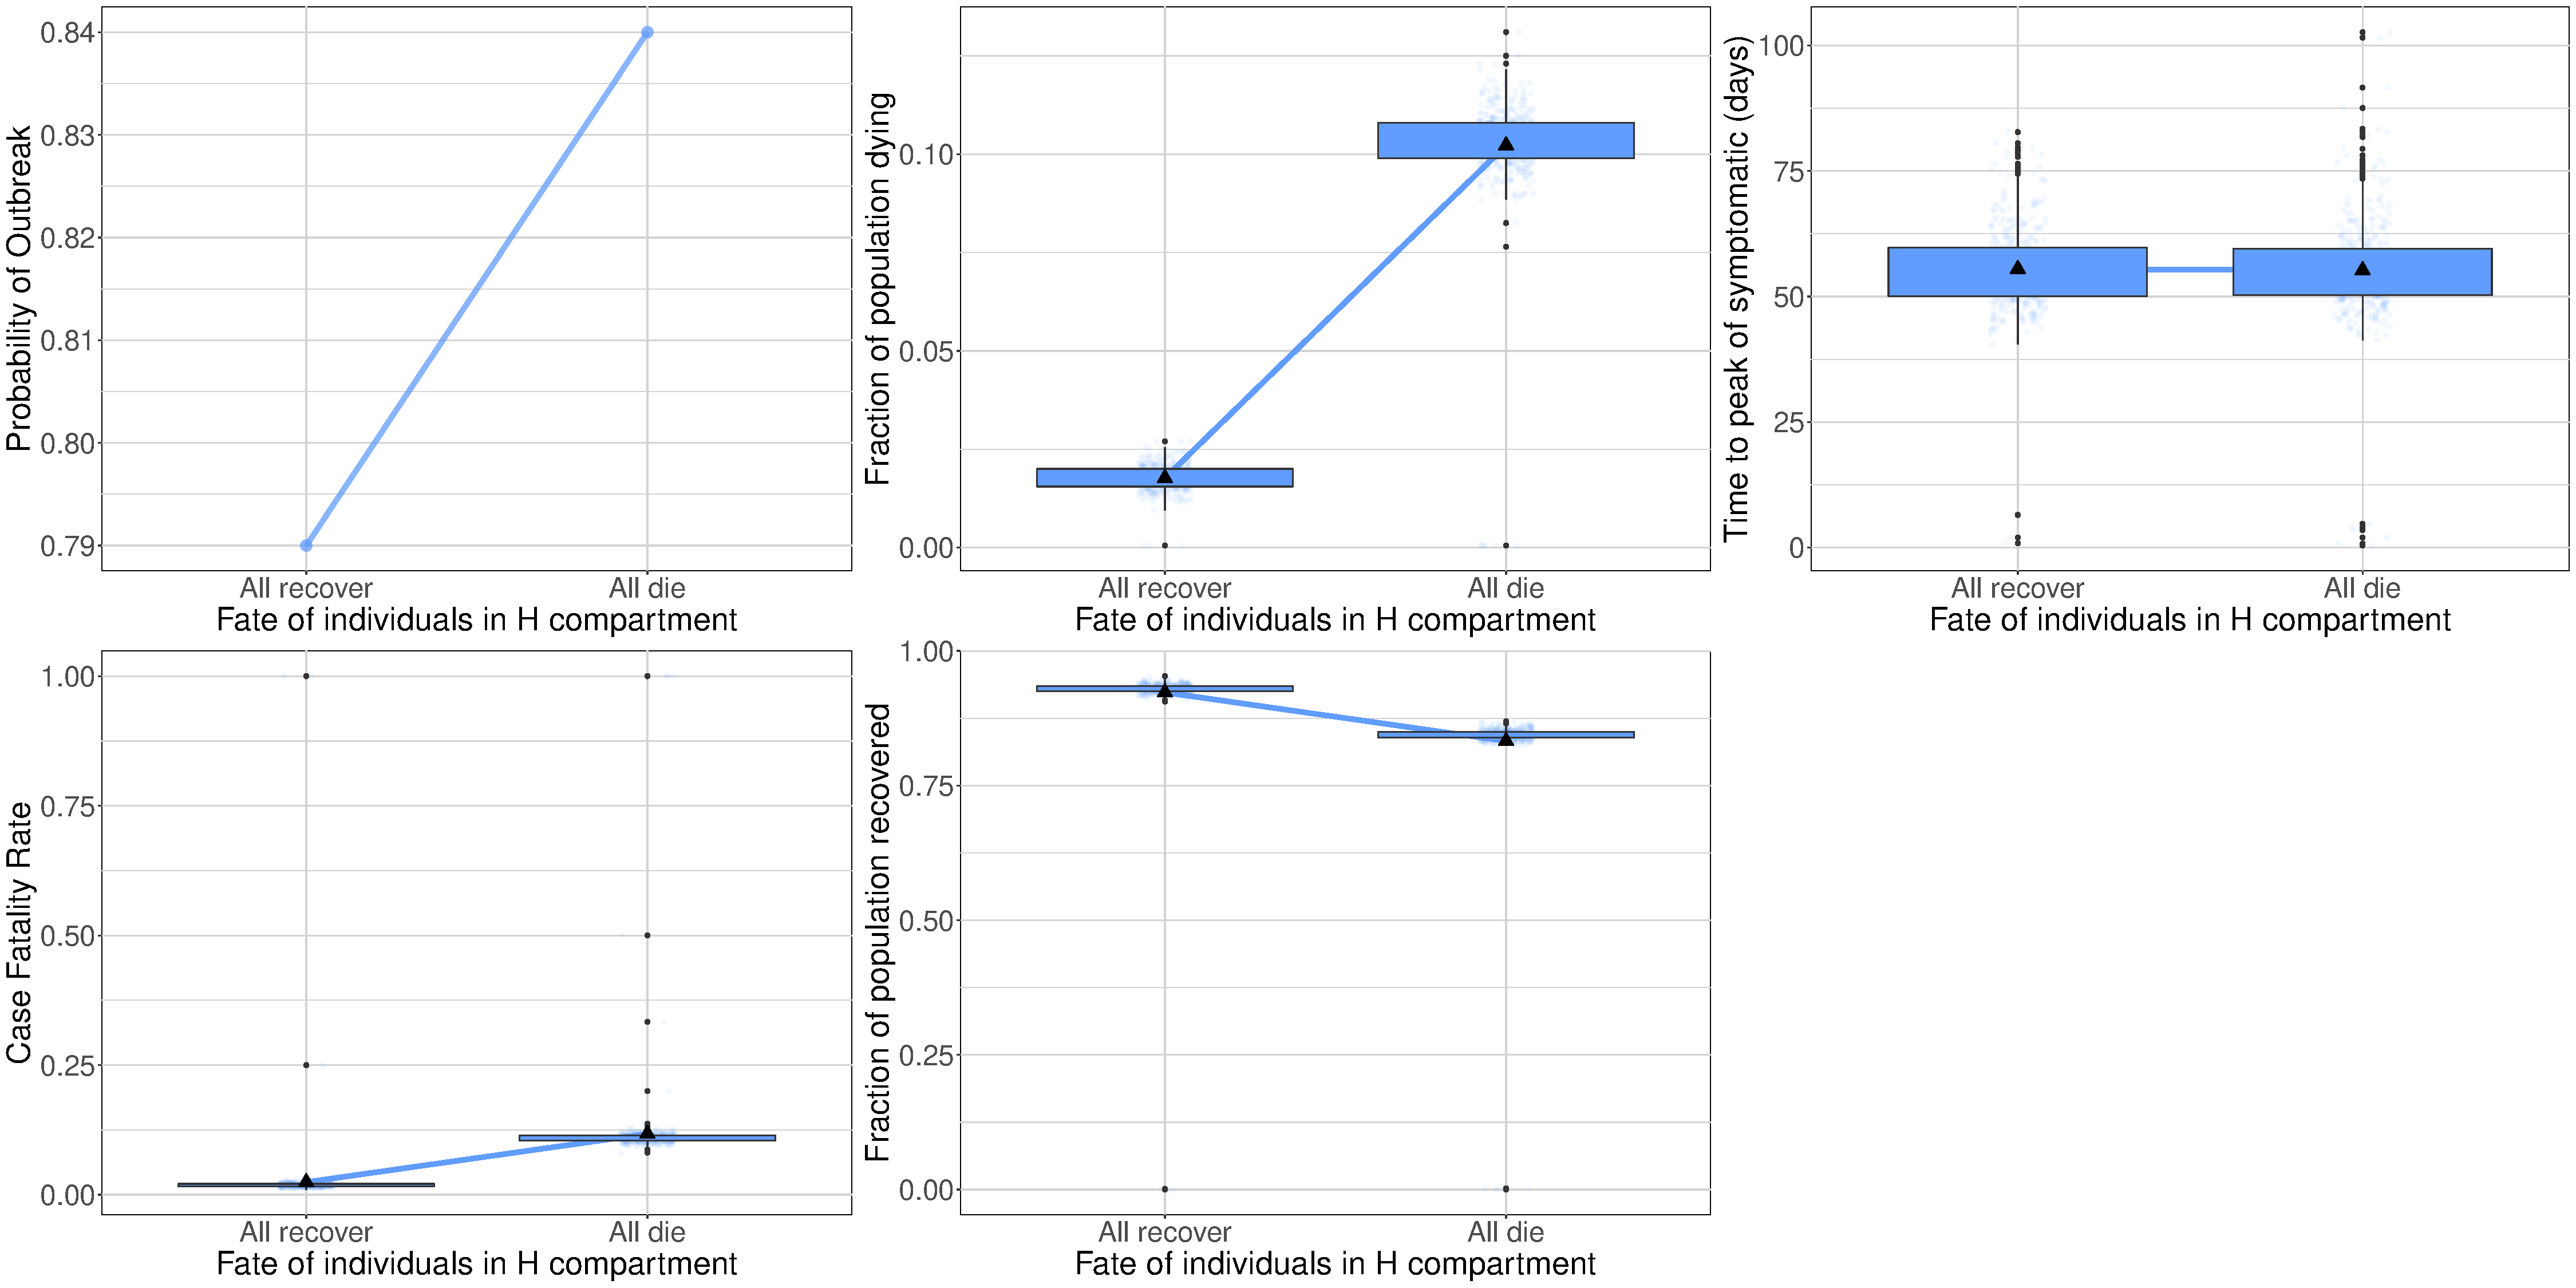
\includegraphics[width=1\textwidth]{figures/FigS2}\hspace{2mm}\caption{\label{fig:Suppl_DvsR} \textbf{Outcomes when all severe (hospitalized)
cases recover ($\sigma=0$) vs when all severe (hospitalized) cases
die ($\sigma=1$).} Probability of an outbreak (top left), fraction
of the population dying (top middle), time until peak symptomatic
cases (top right), IFR (bottom left), and fraction of the population
that recovers (bottom middle). Since we define outbreaks as simulations
in which at least one person dies and probability of a case dying
is higher when $\sigma=1$, the probability of observing an outbreak
is also necessarily higher when$\sigma=1.$}
\end{figure}

\medskip{}

\begin{figure}[H]
\centering{}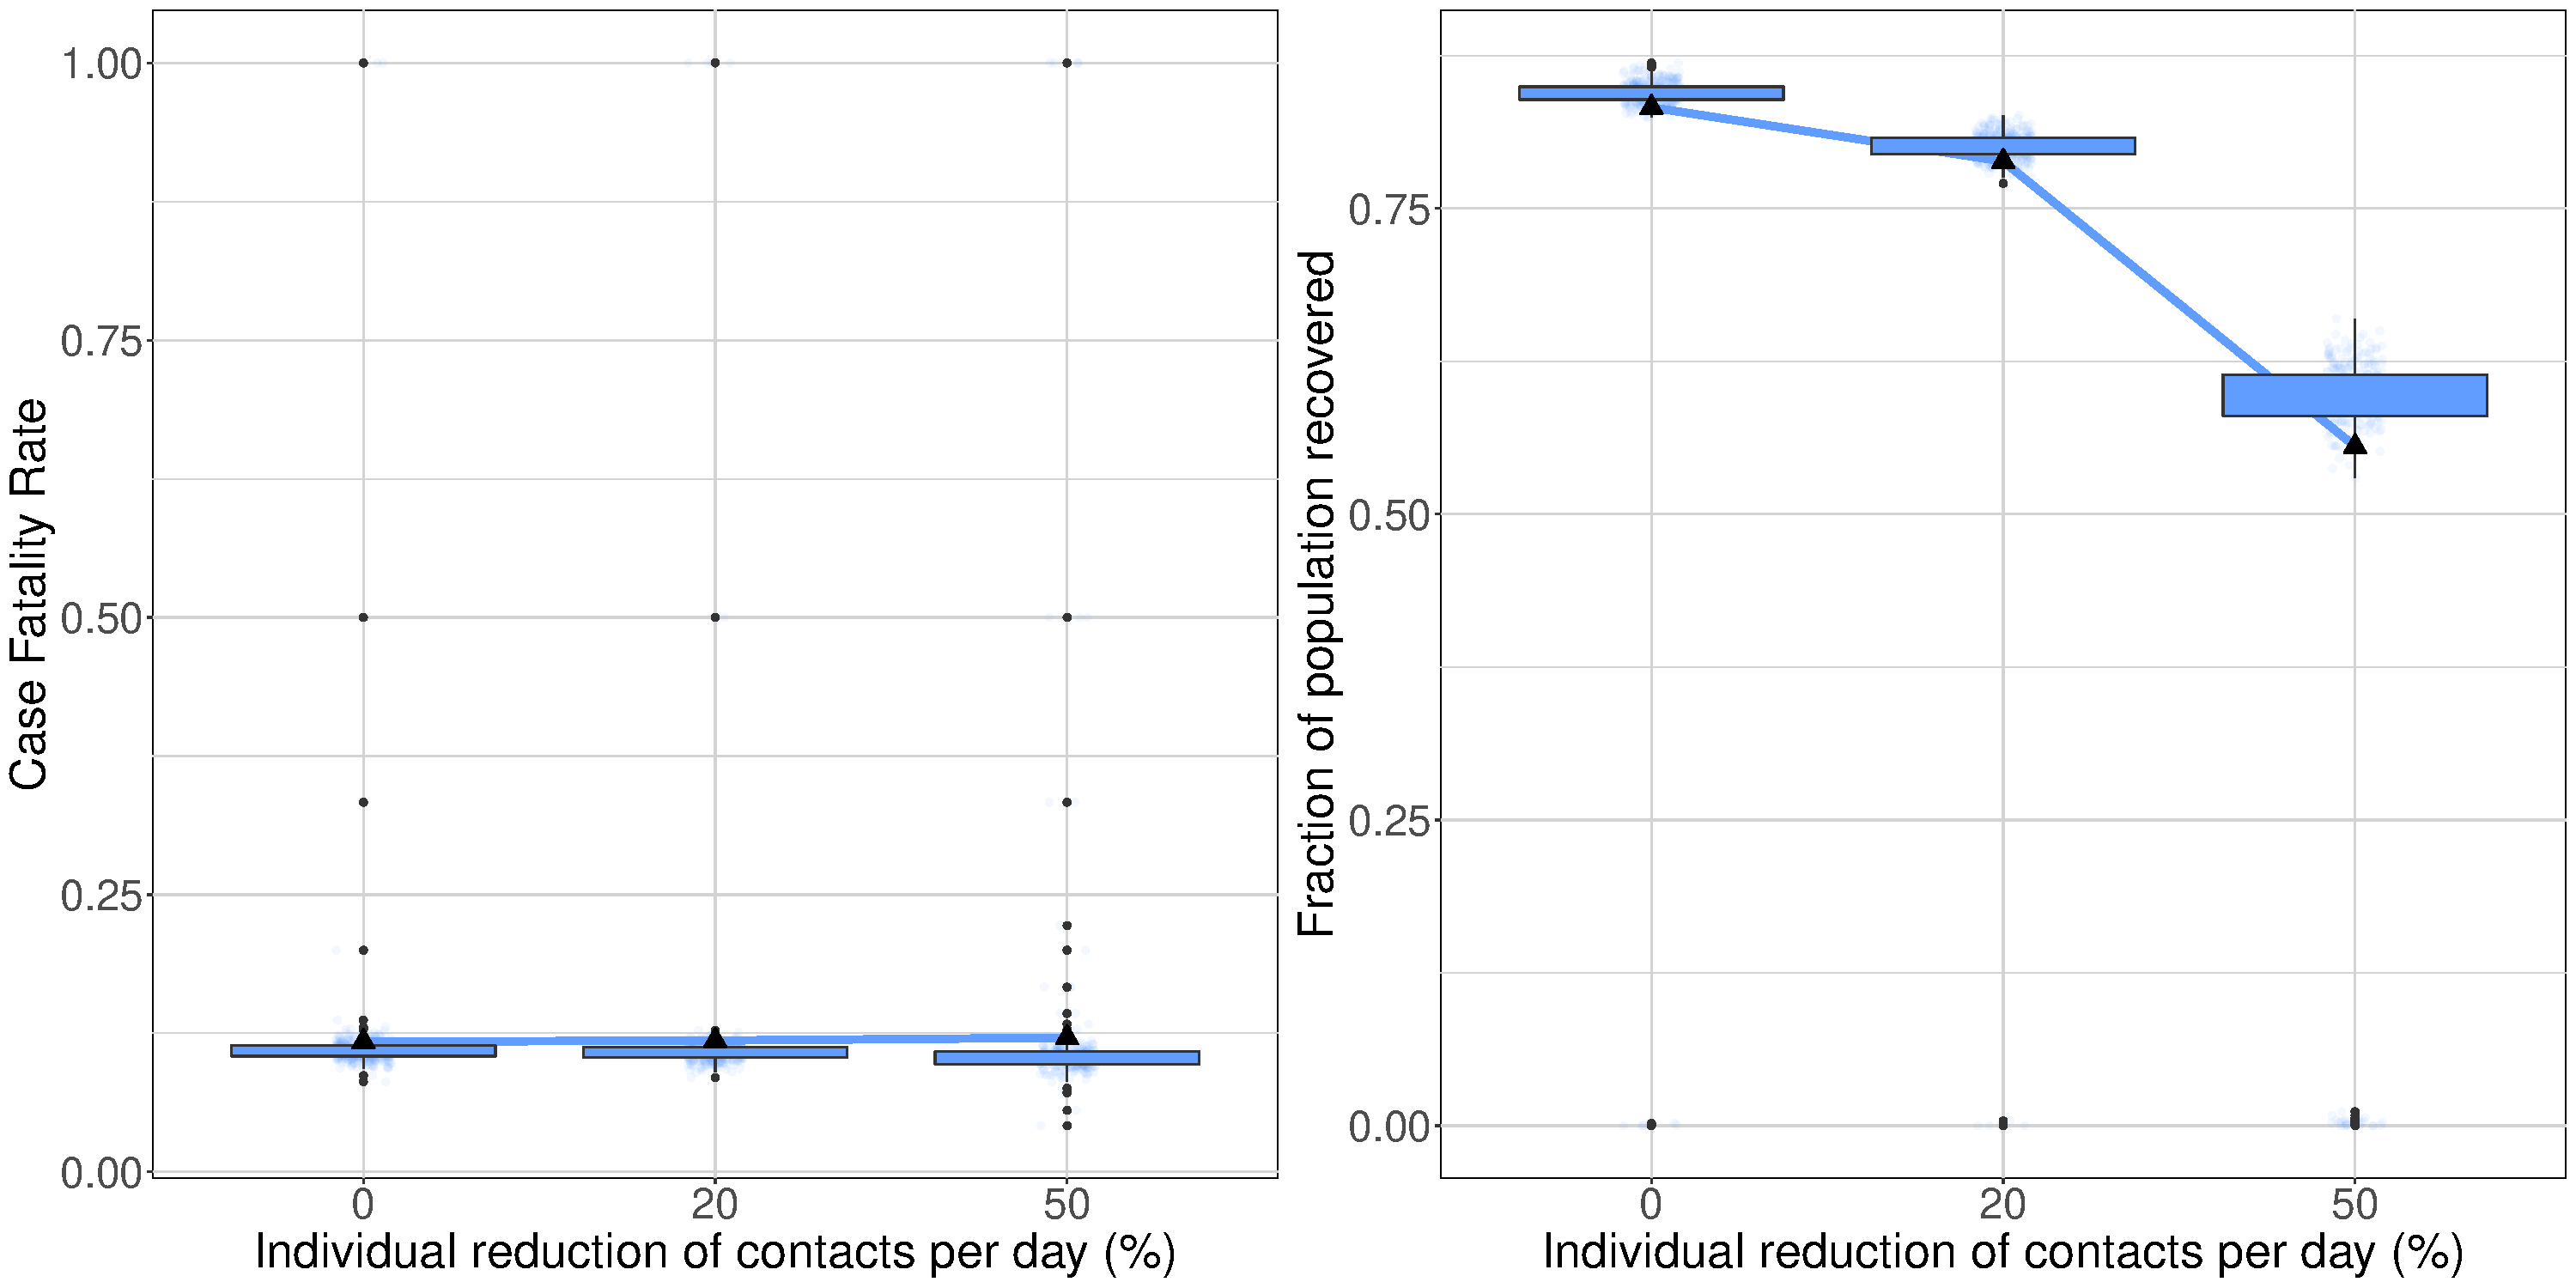
\includegraphics[width=1\textwidth]{figures/FigS3}\hspace{2mm}\caption{\label{fig:Suppl_self} \textbf{Self-distancing.} IFR (left), and
fraction of the population that recovers (right) as a function of
the proportion of contacts reduced per individual per day.}
\end{figure}
\medskip{}

\begin{figure}[H]
\centering{}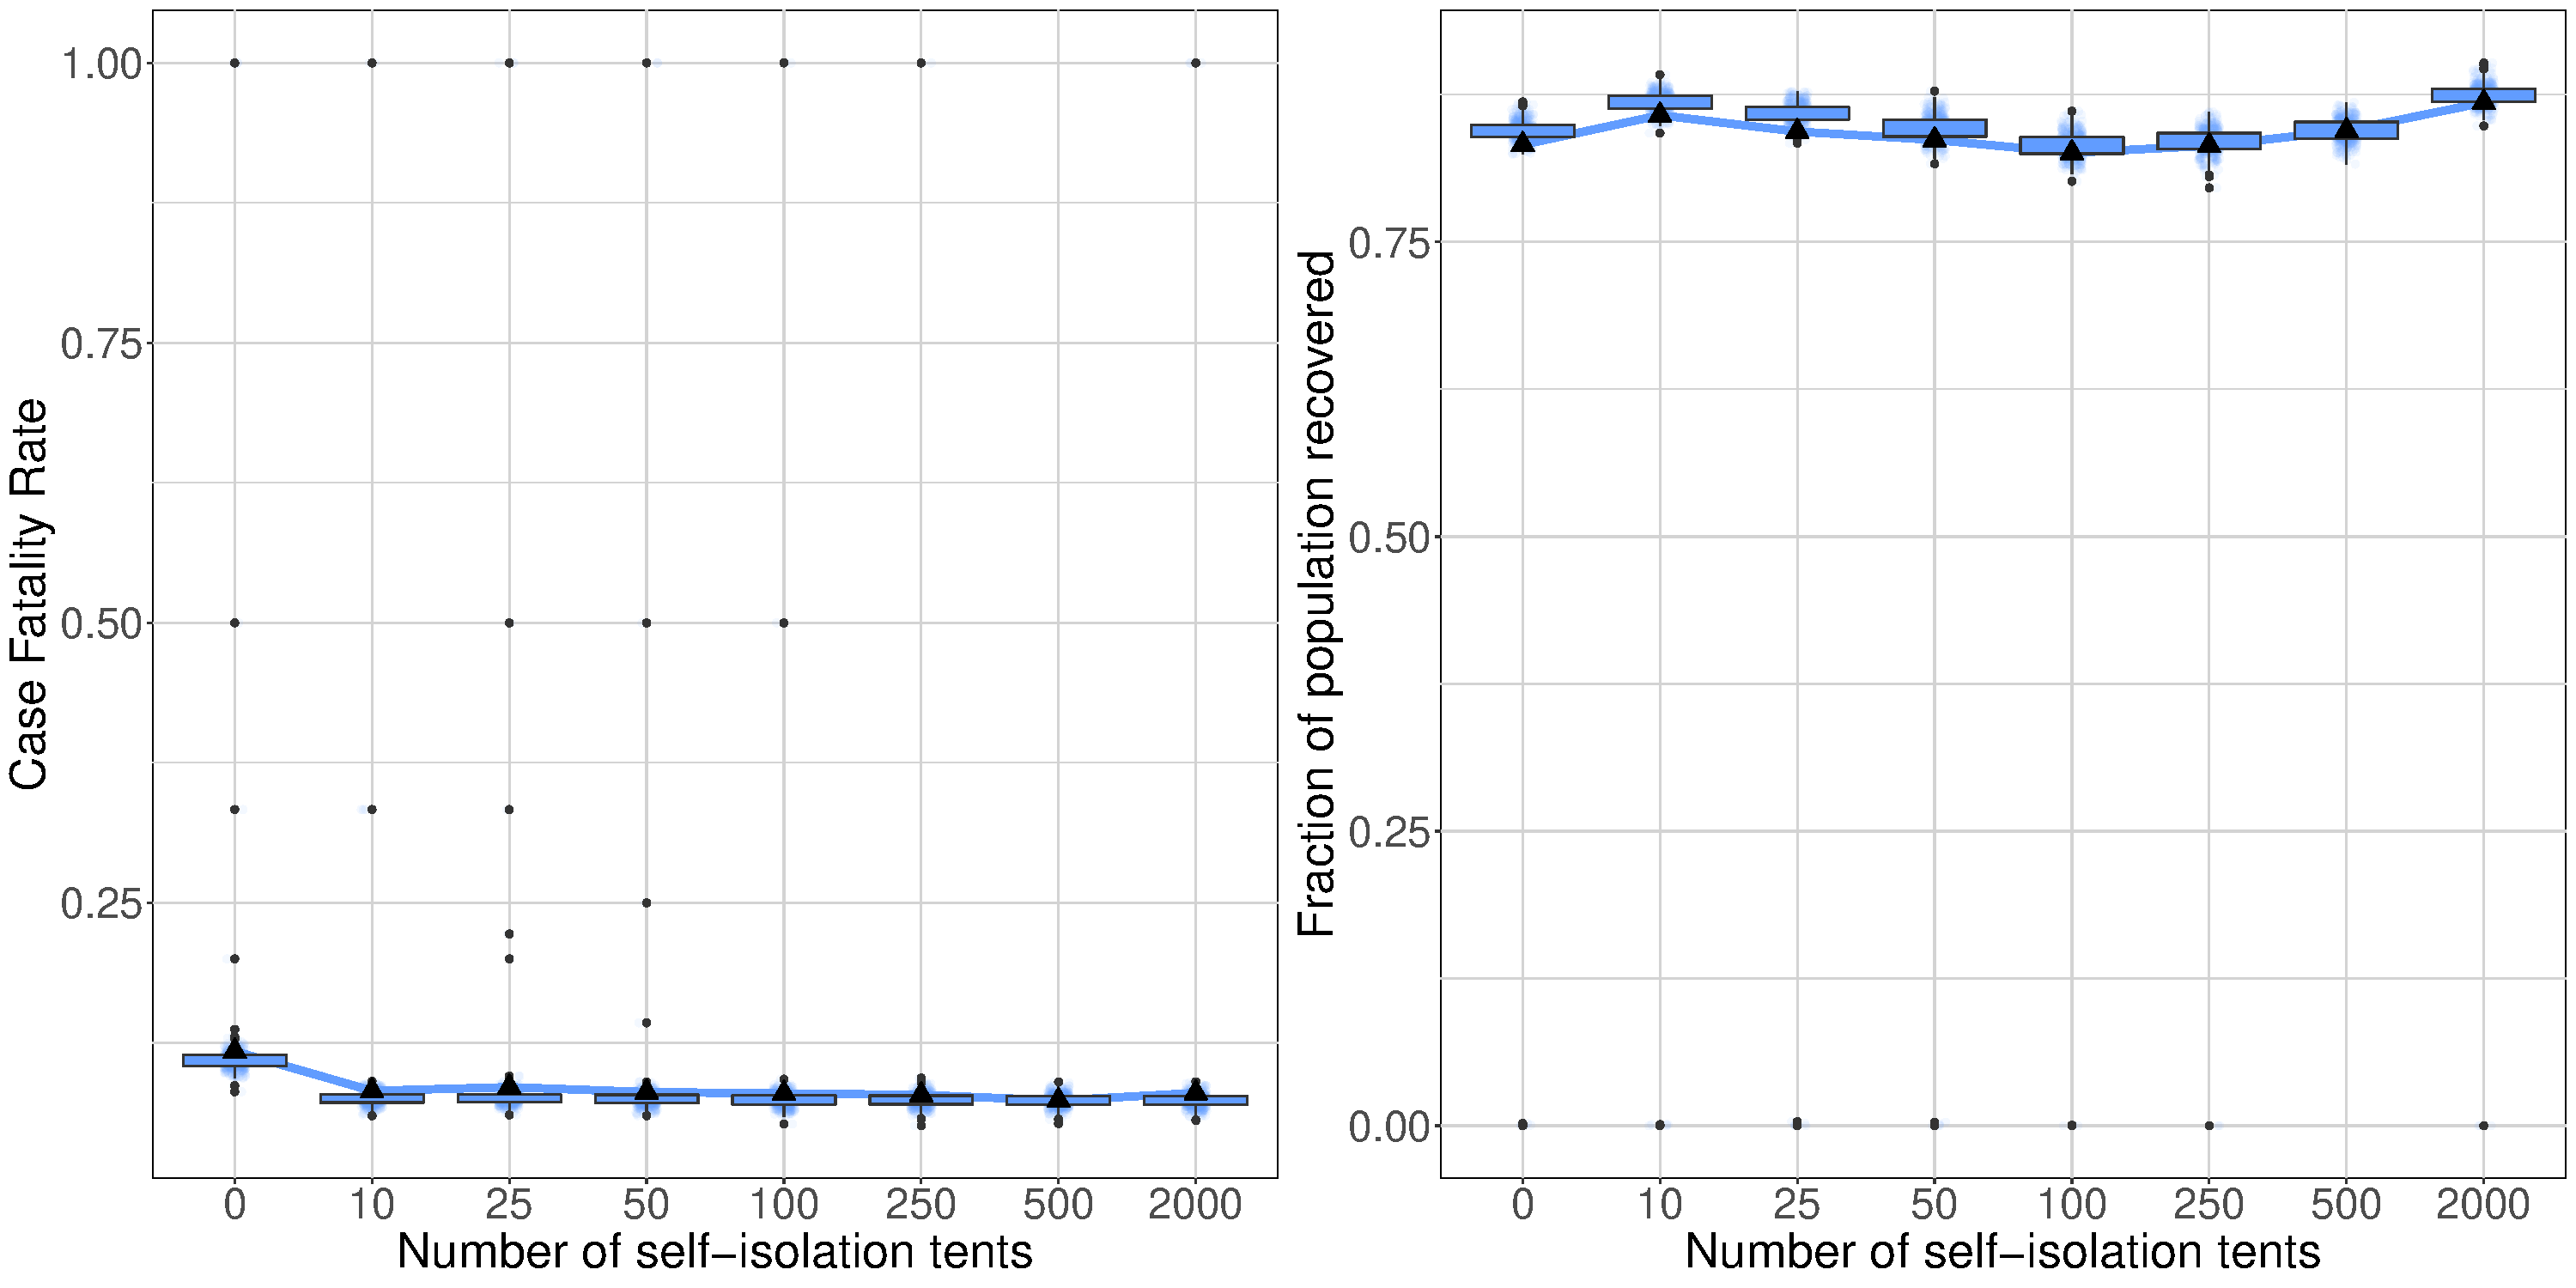
\includegraphics[width=1\textwidth]{figures/FigS4}\hspace{2mm}\caption{\label{fig:Suppl_isolation} \textbf{Self-isolation.} IFR (left),
and fraction of the population that recovers (right) as a function
of the number of isolation tents available in the camp.}
\end{figure}

\medskip{}

\begin{figure}[H]
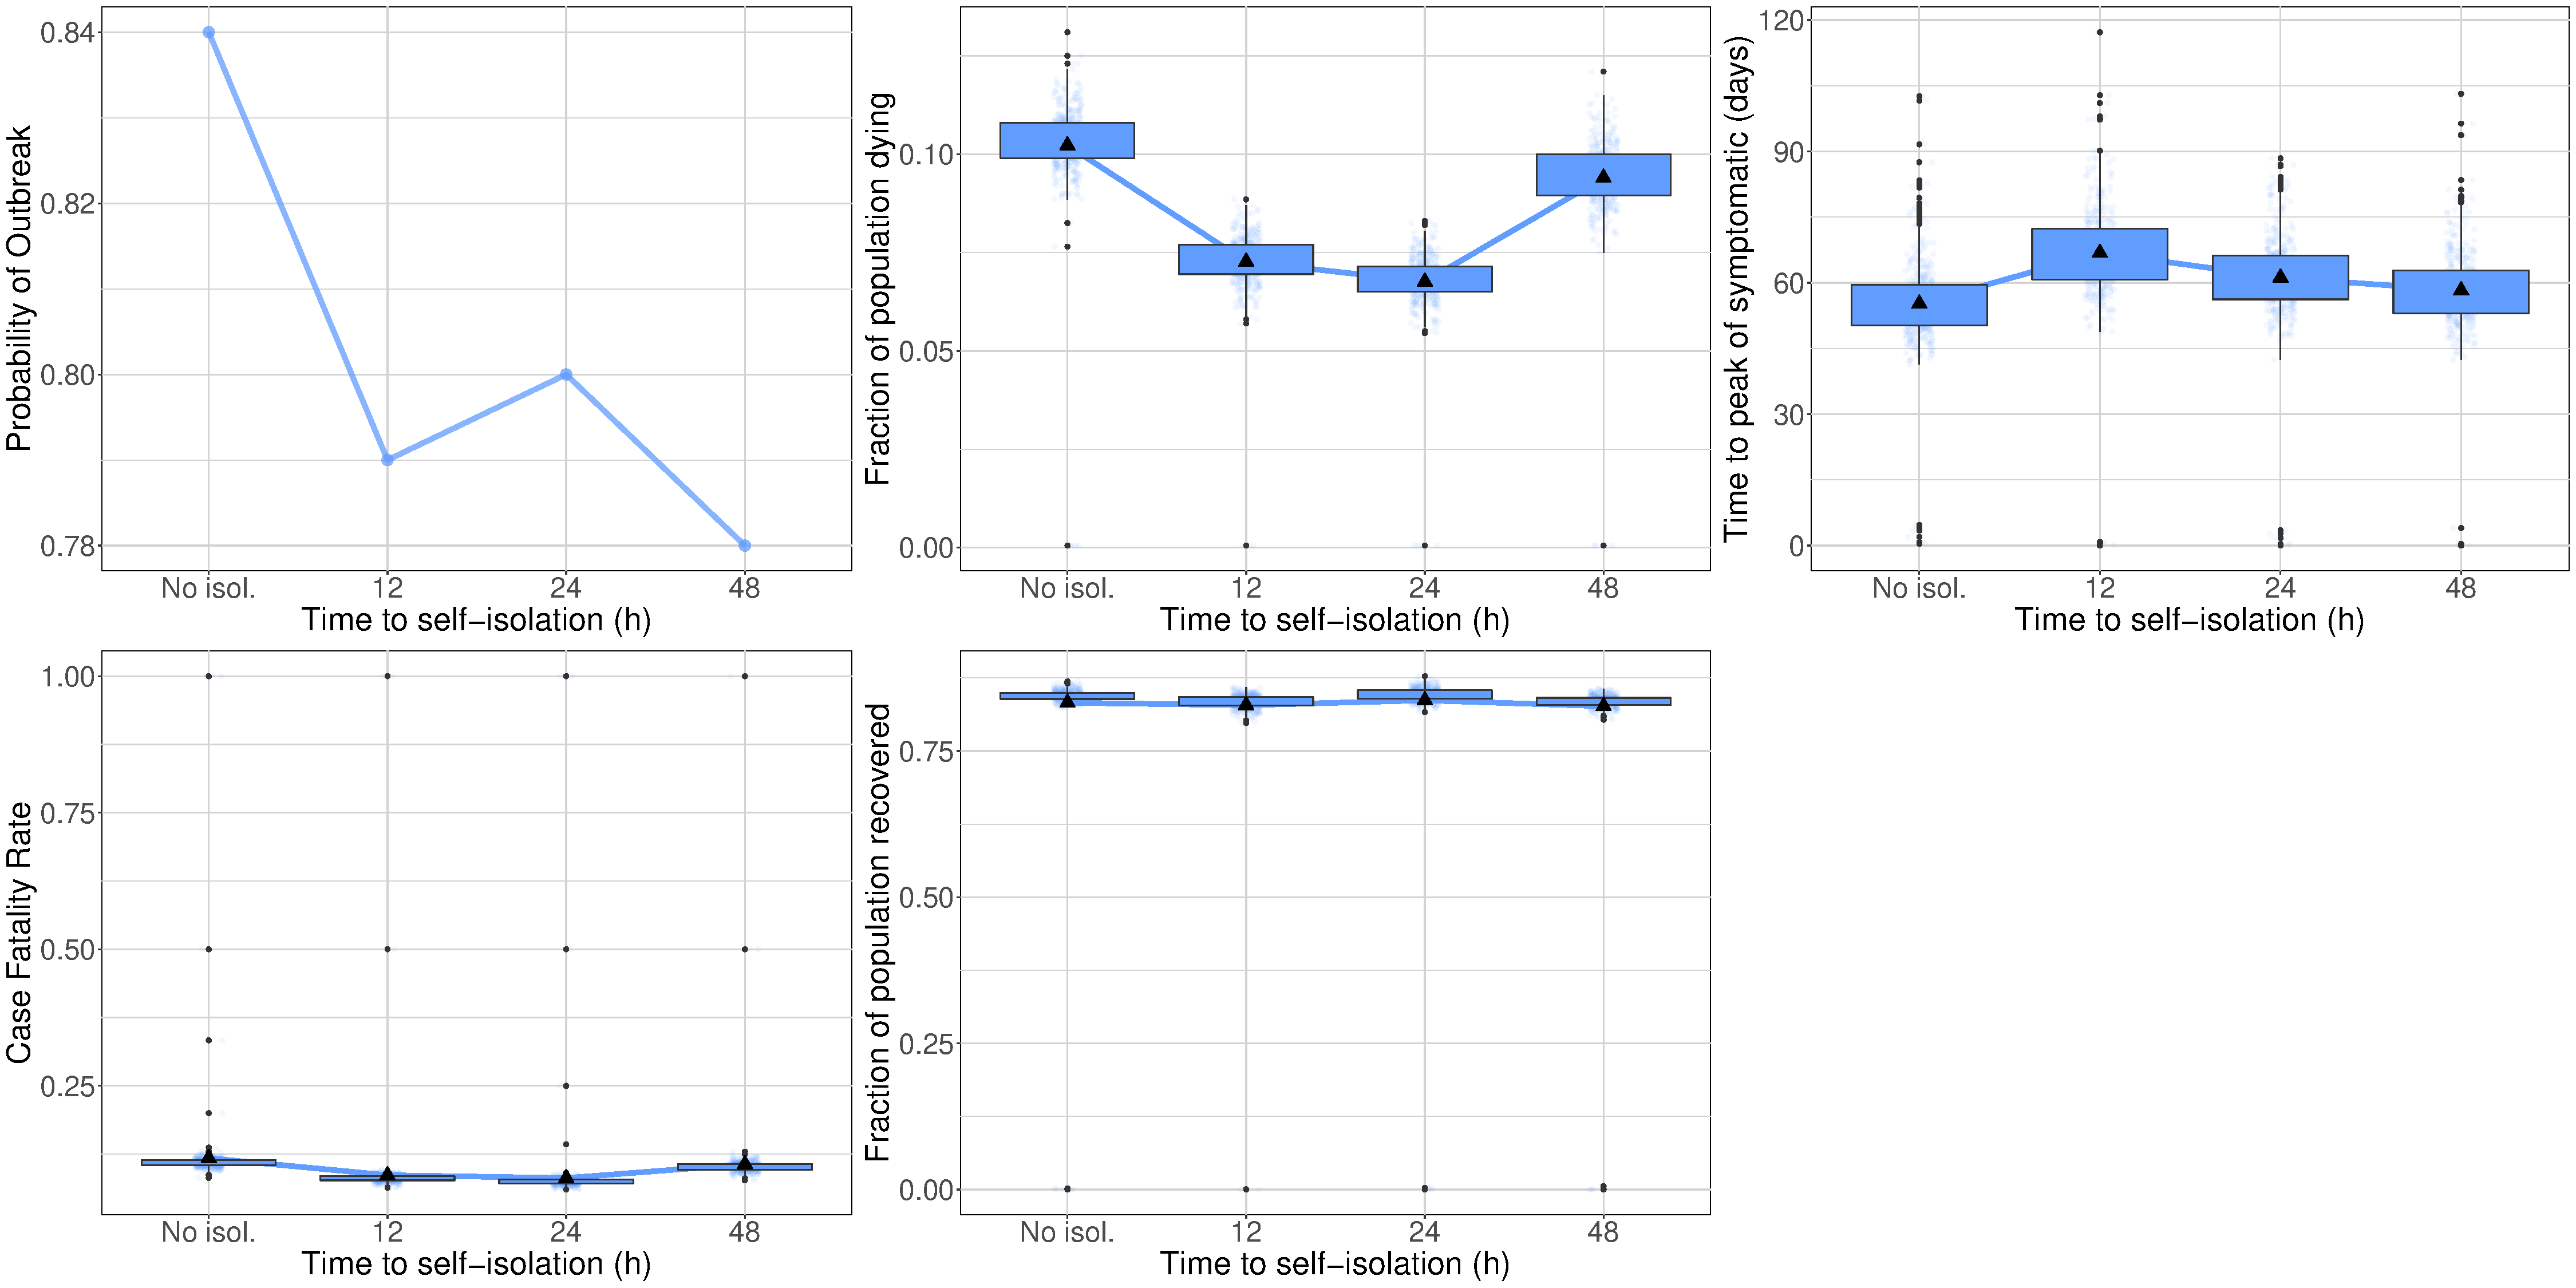
\includegraphics[width=1\textwidth]{figures/FigS5}\hspace{2mm}\caption{\label{fig:Suppl_onset} \textbf{Time to self-isolation.} Probability
of an outbreak (top left), fraction of the population dying (top middle),
time until peak symptomatic cases (top right), IFR (bottom left),
and fraction of the population that recovers (bottom middle) as a
function of the time that individuals require to recognize their symptoms
and self-isolate. The isolation capacity }
\end{figure}

\medskip{}

\begin{figure}[H]
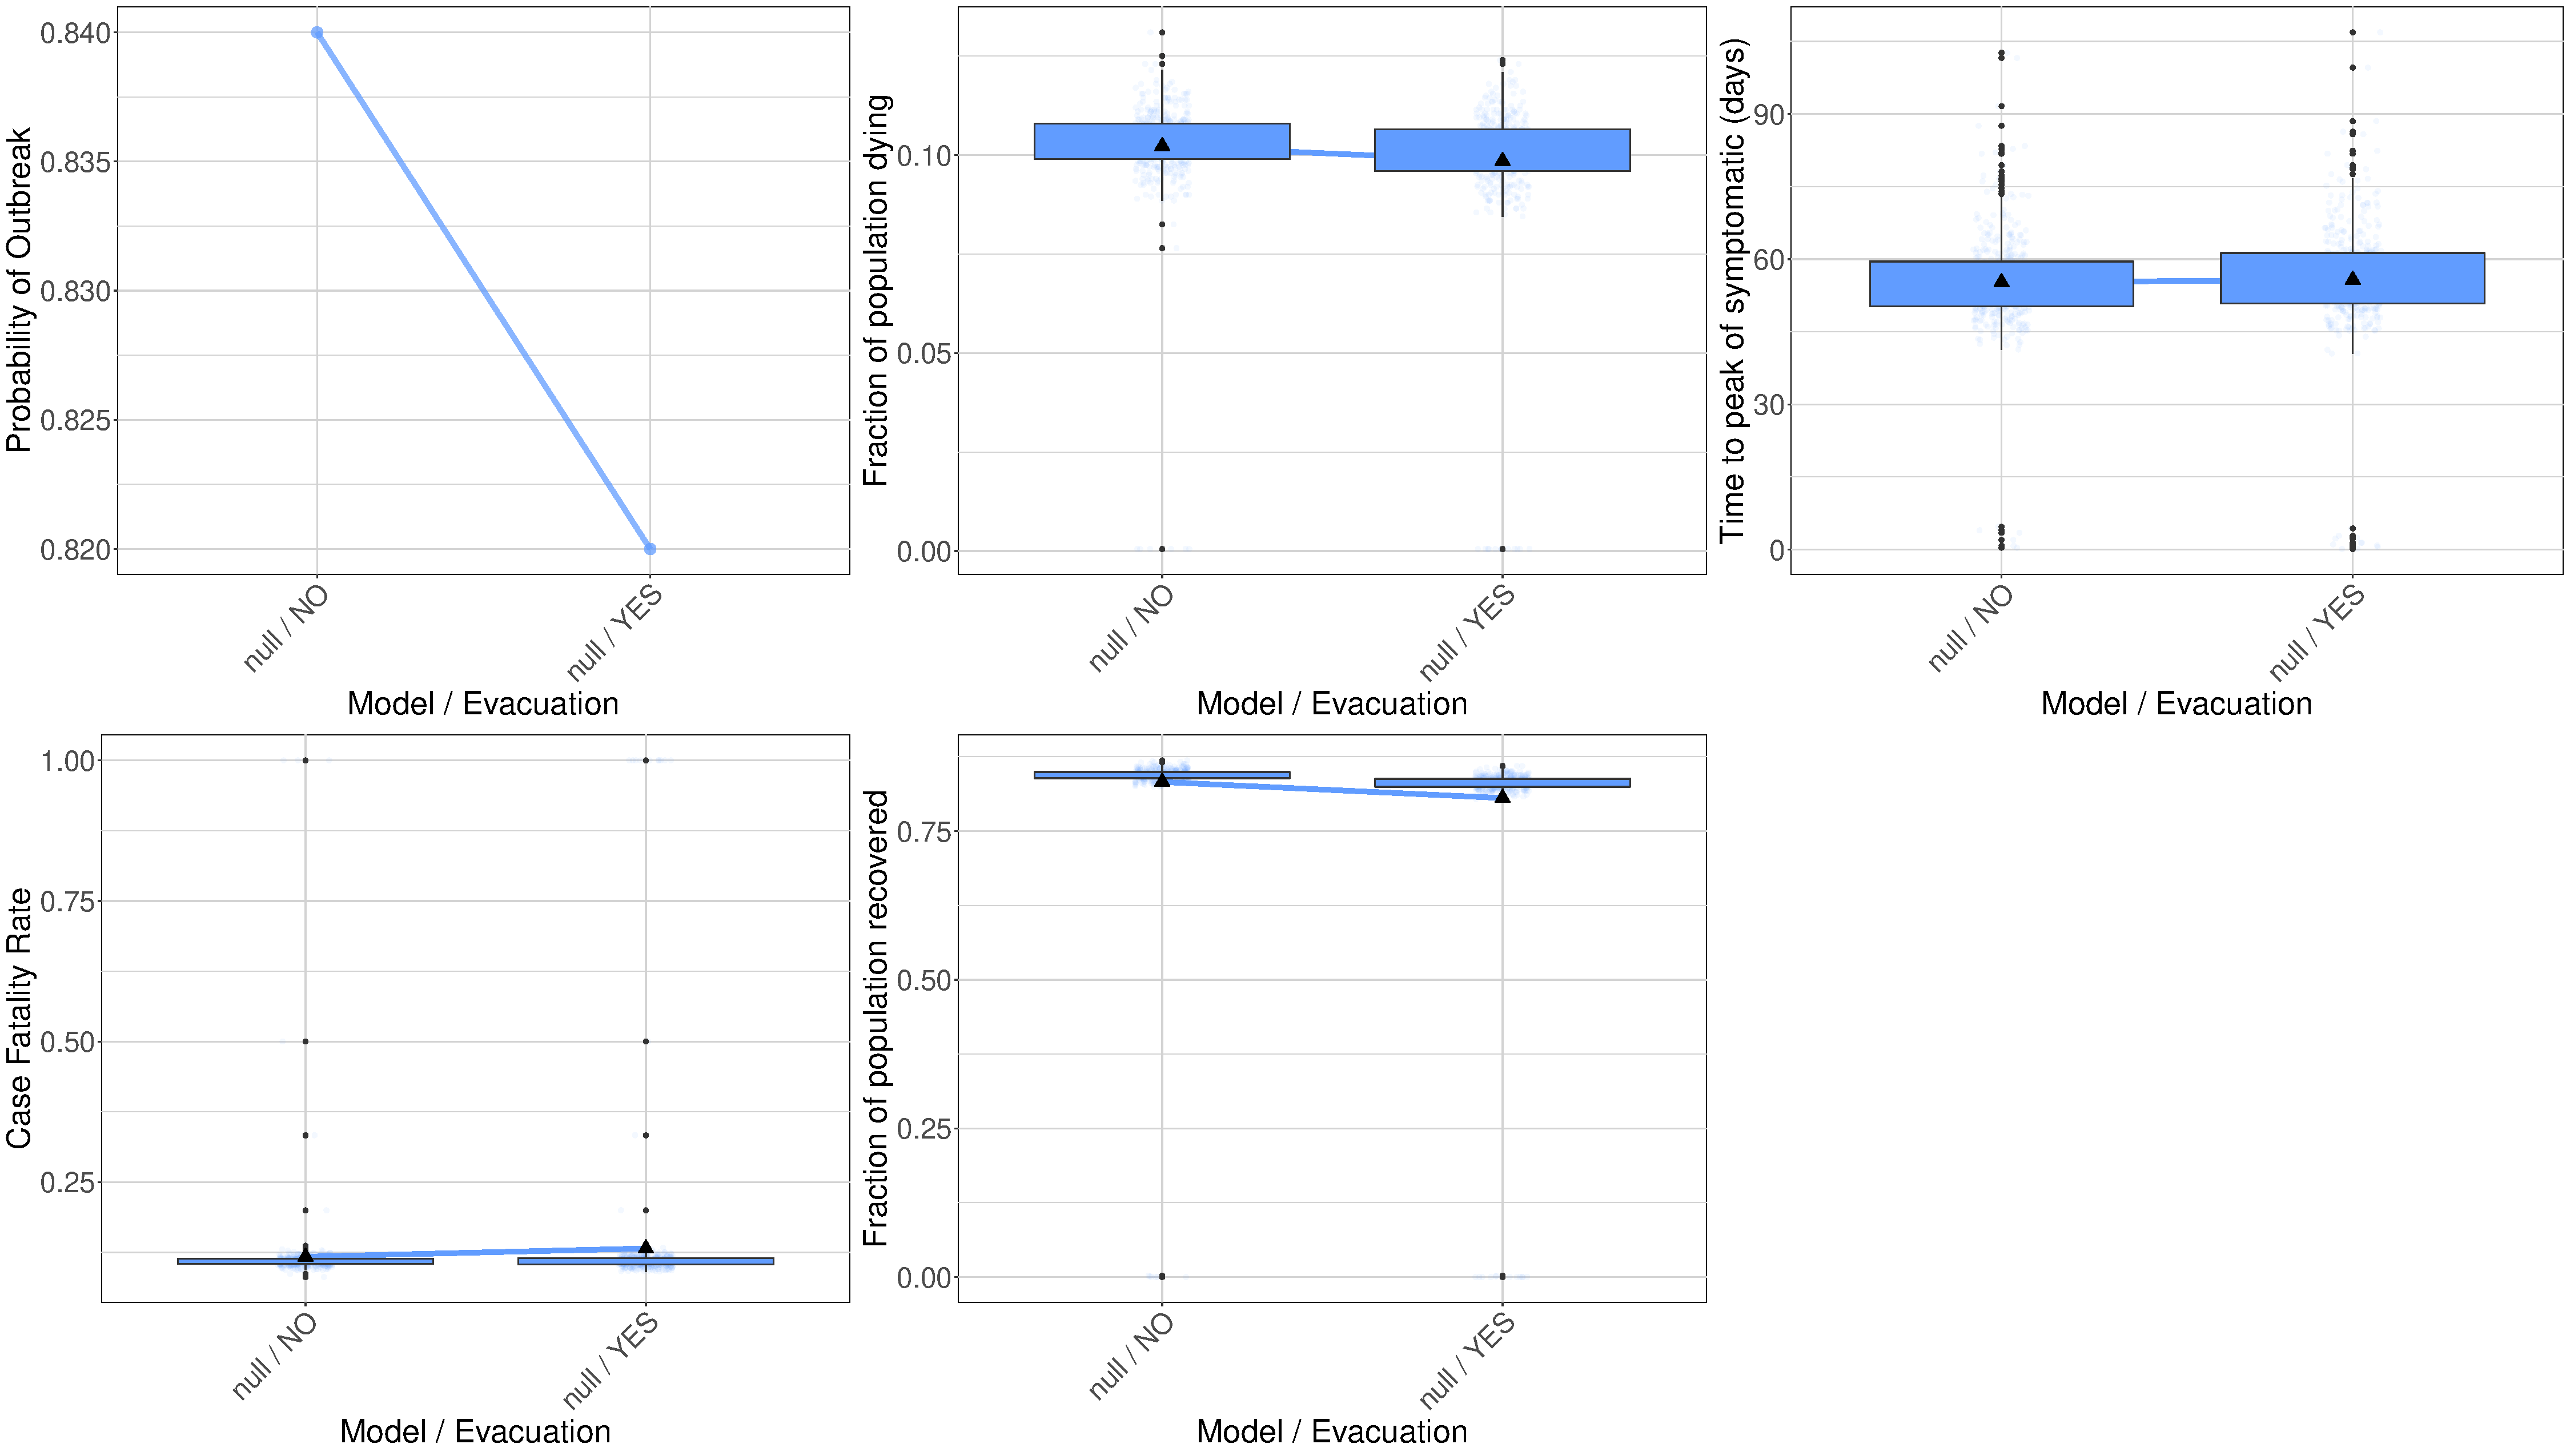
\includegraphics[width=1\textwidth]{figures/FigS6}\hspace{2mm}\caption{\label{fig:Suppl_evacuation} \textbf{Evacuation.} Probability of
an outbreak (top left), fraction of the population dying (top middle),
time until peak symptomatic cases (top right), IFR (bottom left),
and fraction of the population that recovers (bottom middle), as a
function of whether individuals requiring hospitalization are evacuated
to isolation centers.}
\end{figure}

\medskip{}

\begin{figure}[H]
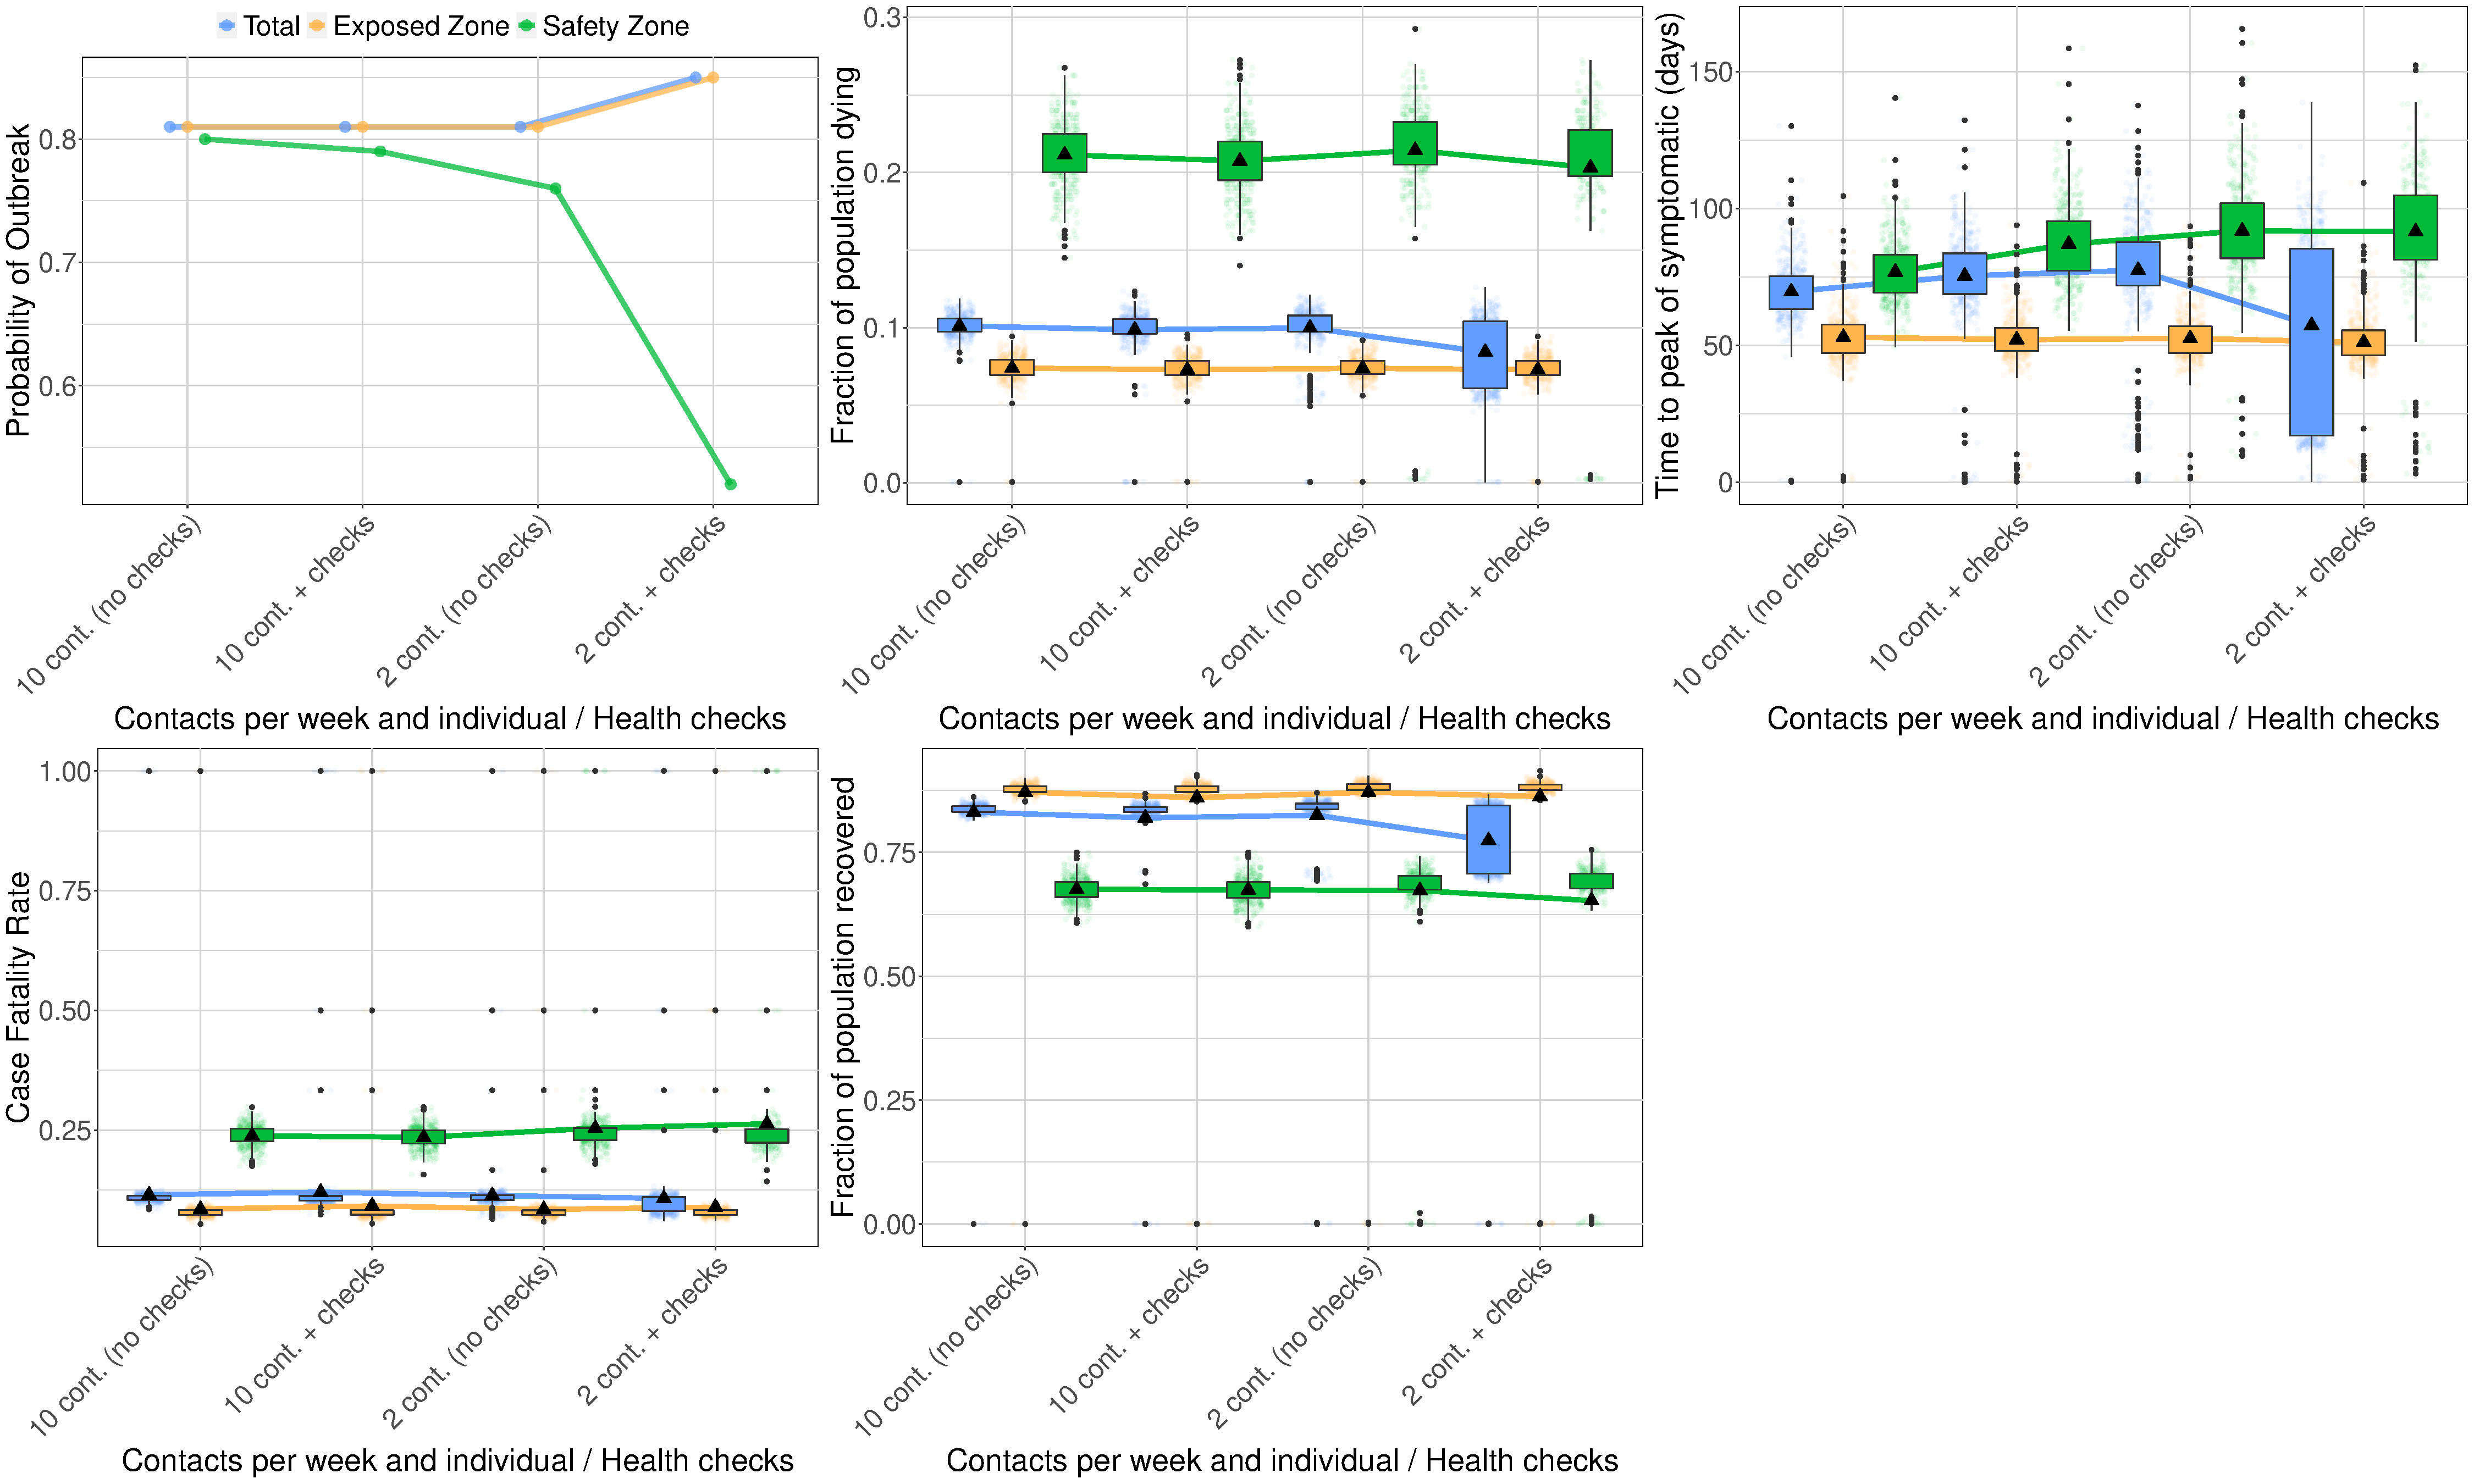
\includegraphics[width=1\textwidth]{figures/FigS7}\hspace{2mm}\caption{\label{fig:Suppl_Tcheck} \textbf{Health-checks in the buffer zone.}
Probability of an outbreak (top left), fraction of the population
dying (top middle), time until peak symptomatic cases (top right),
IFR (bottom left), and fraction of the population that recovers (bottom
middle), as a function of whether health-checks are implemented in
the buffer zone between the safety and exposed zones. Scenarios with
10 or 2 contacts in the buffer zone per person in the safety zone
per week are plotted. All figures consider the scenario in which 20\%
of the camp's population is allocated to the safety zone.}
\end{figure}

\begin{figure}[H]
\centering{}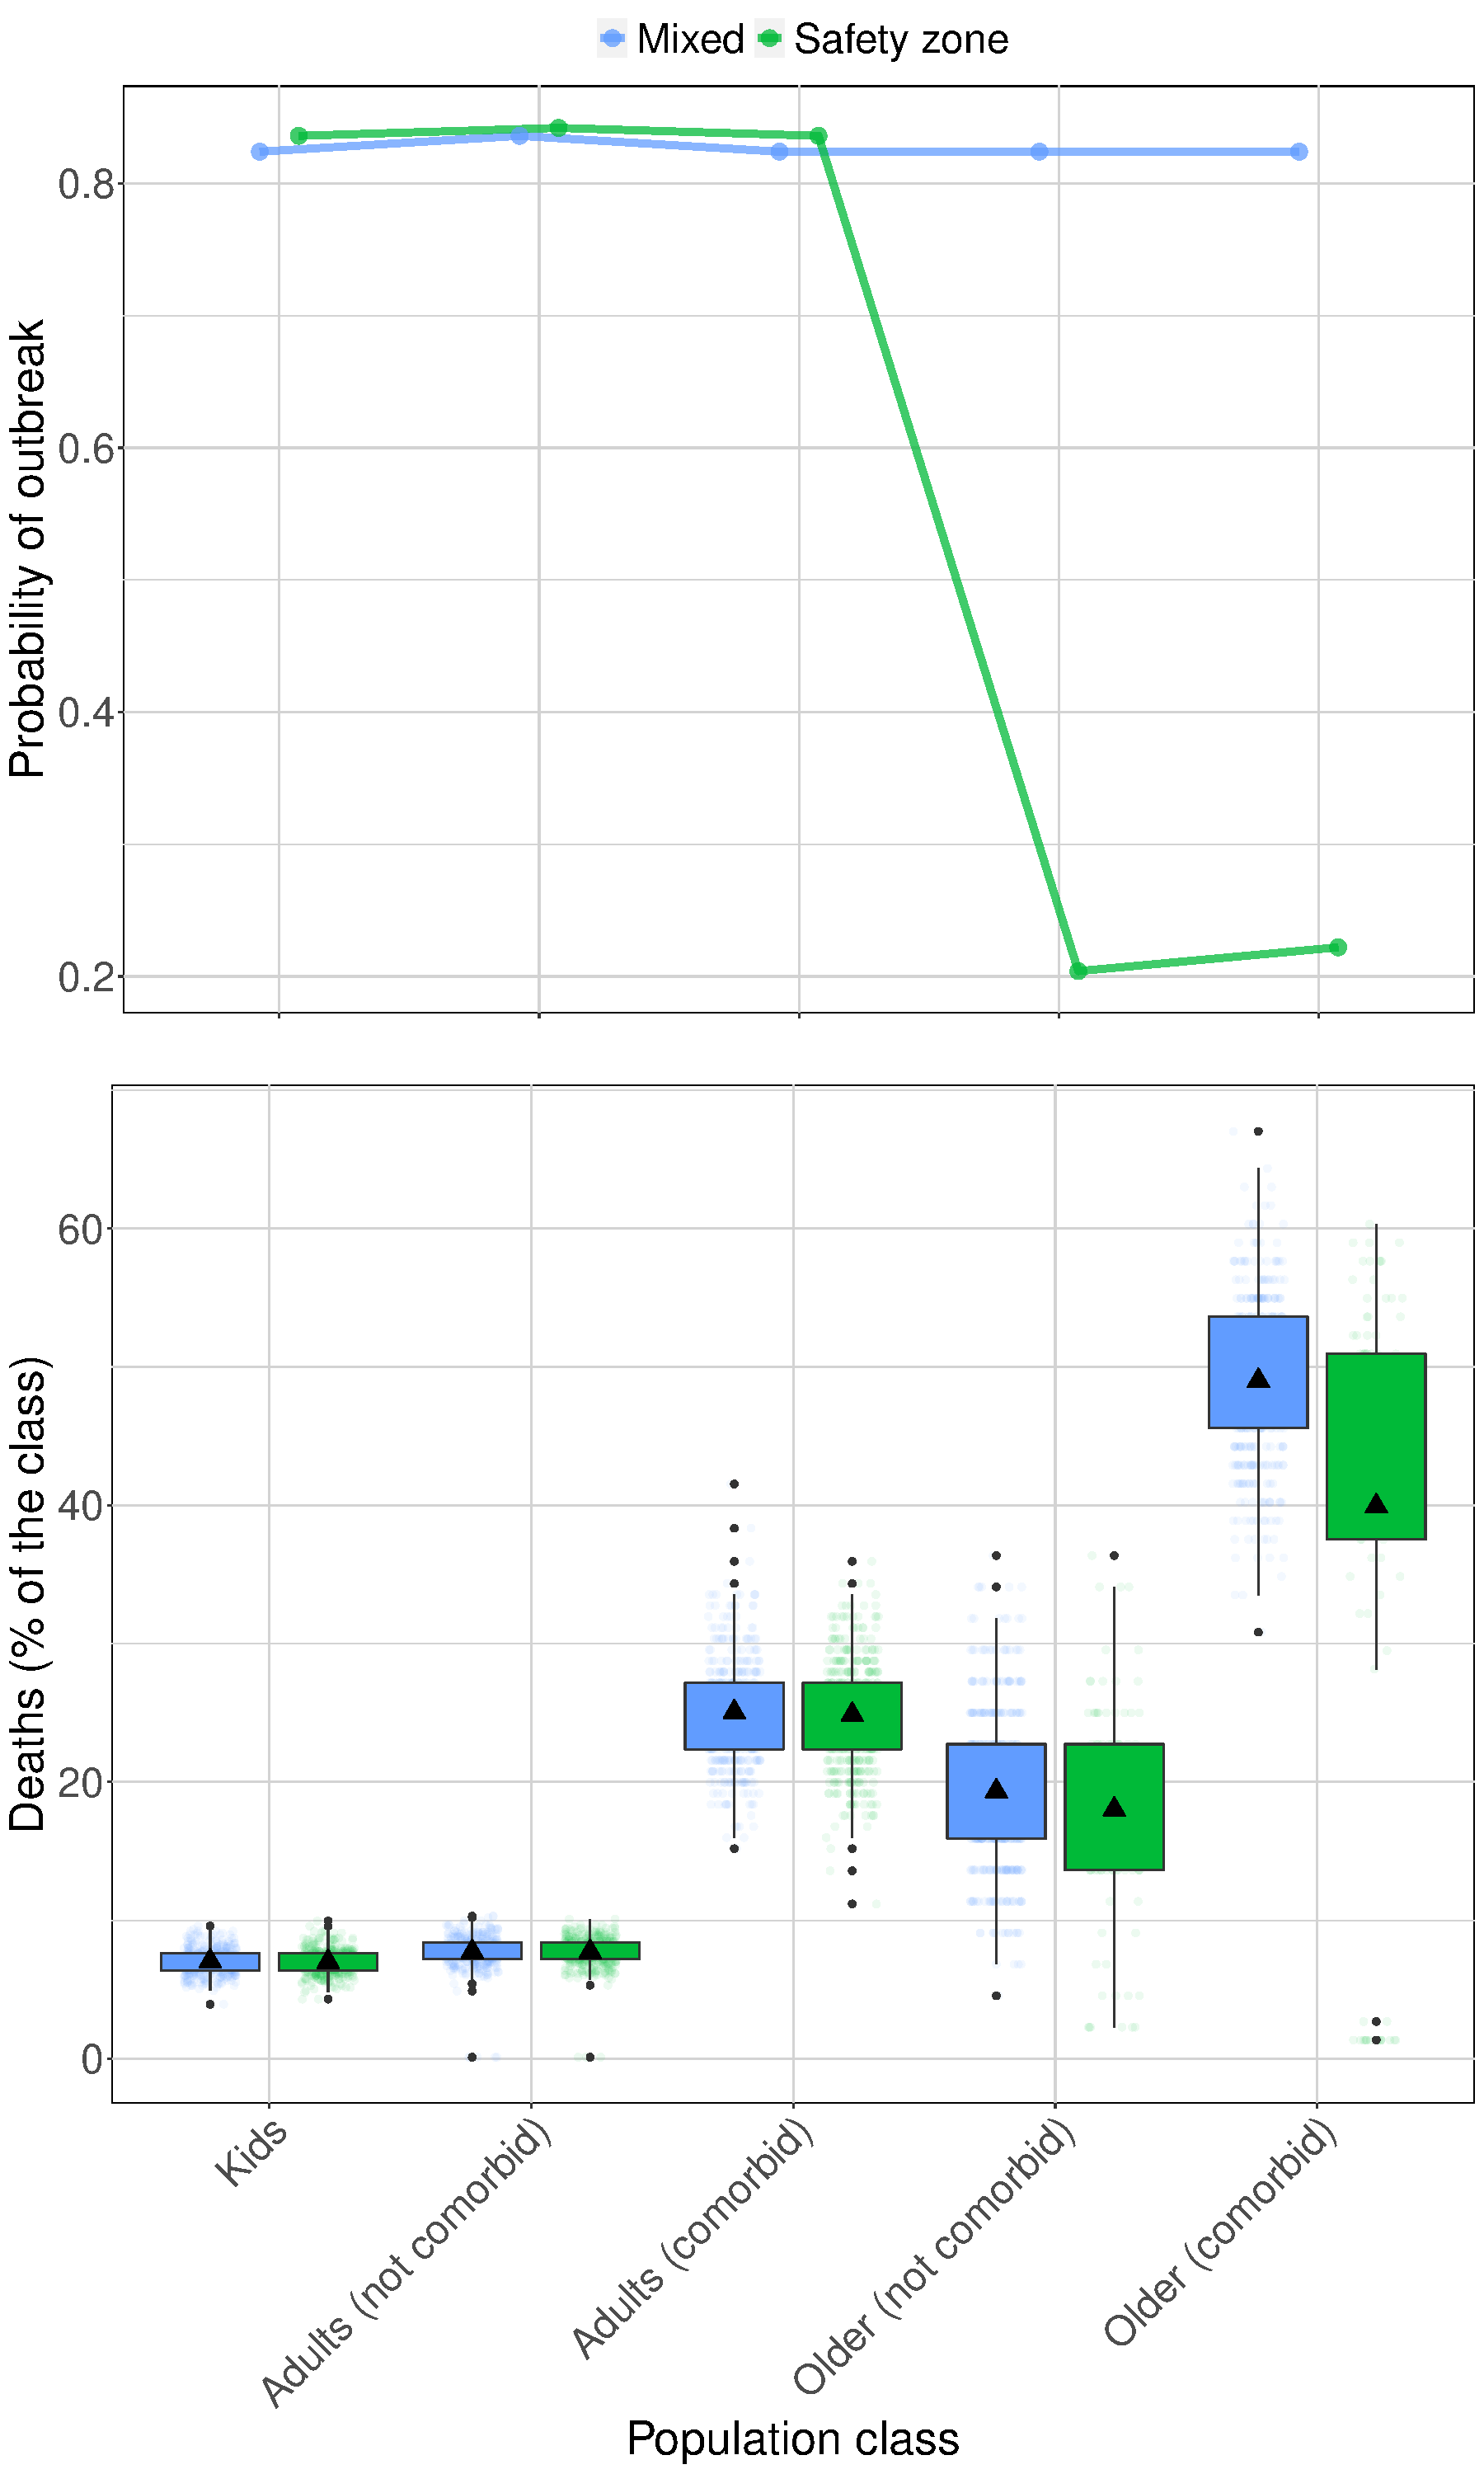
\includegraphics[width=0.6\textwidth]{figures/FigS8}\hspace{2mm}\caption{\label{fig:Suppl_agegroups} \textbf{Effects of the safety zone on
outcomes by population class. }Probability of an outbreak (top), and
proportion that dies in each population class (bottom) when no interventions
are implemented (Mixed), compared to protection of older adults in
the safety zone with 2 contacts in the buffer zone per week (Safety
zone). The fraction of deaths in the safety zone for the older population
is significantly lower (Kruskal-Wallis test, p-val$<10^{-15}$).}
\end{figure}
\medskip{}

\begin{figure}[H]
\centering{}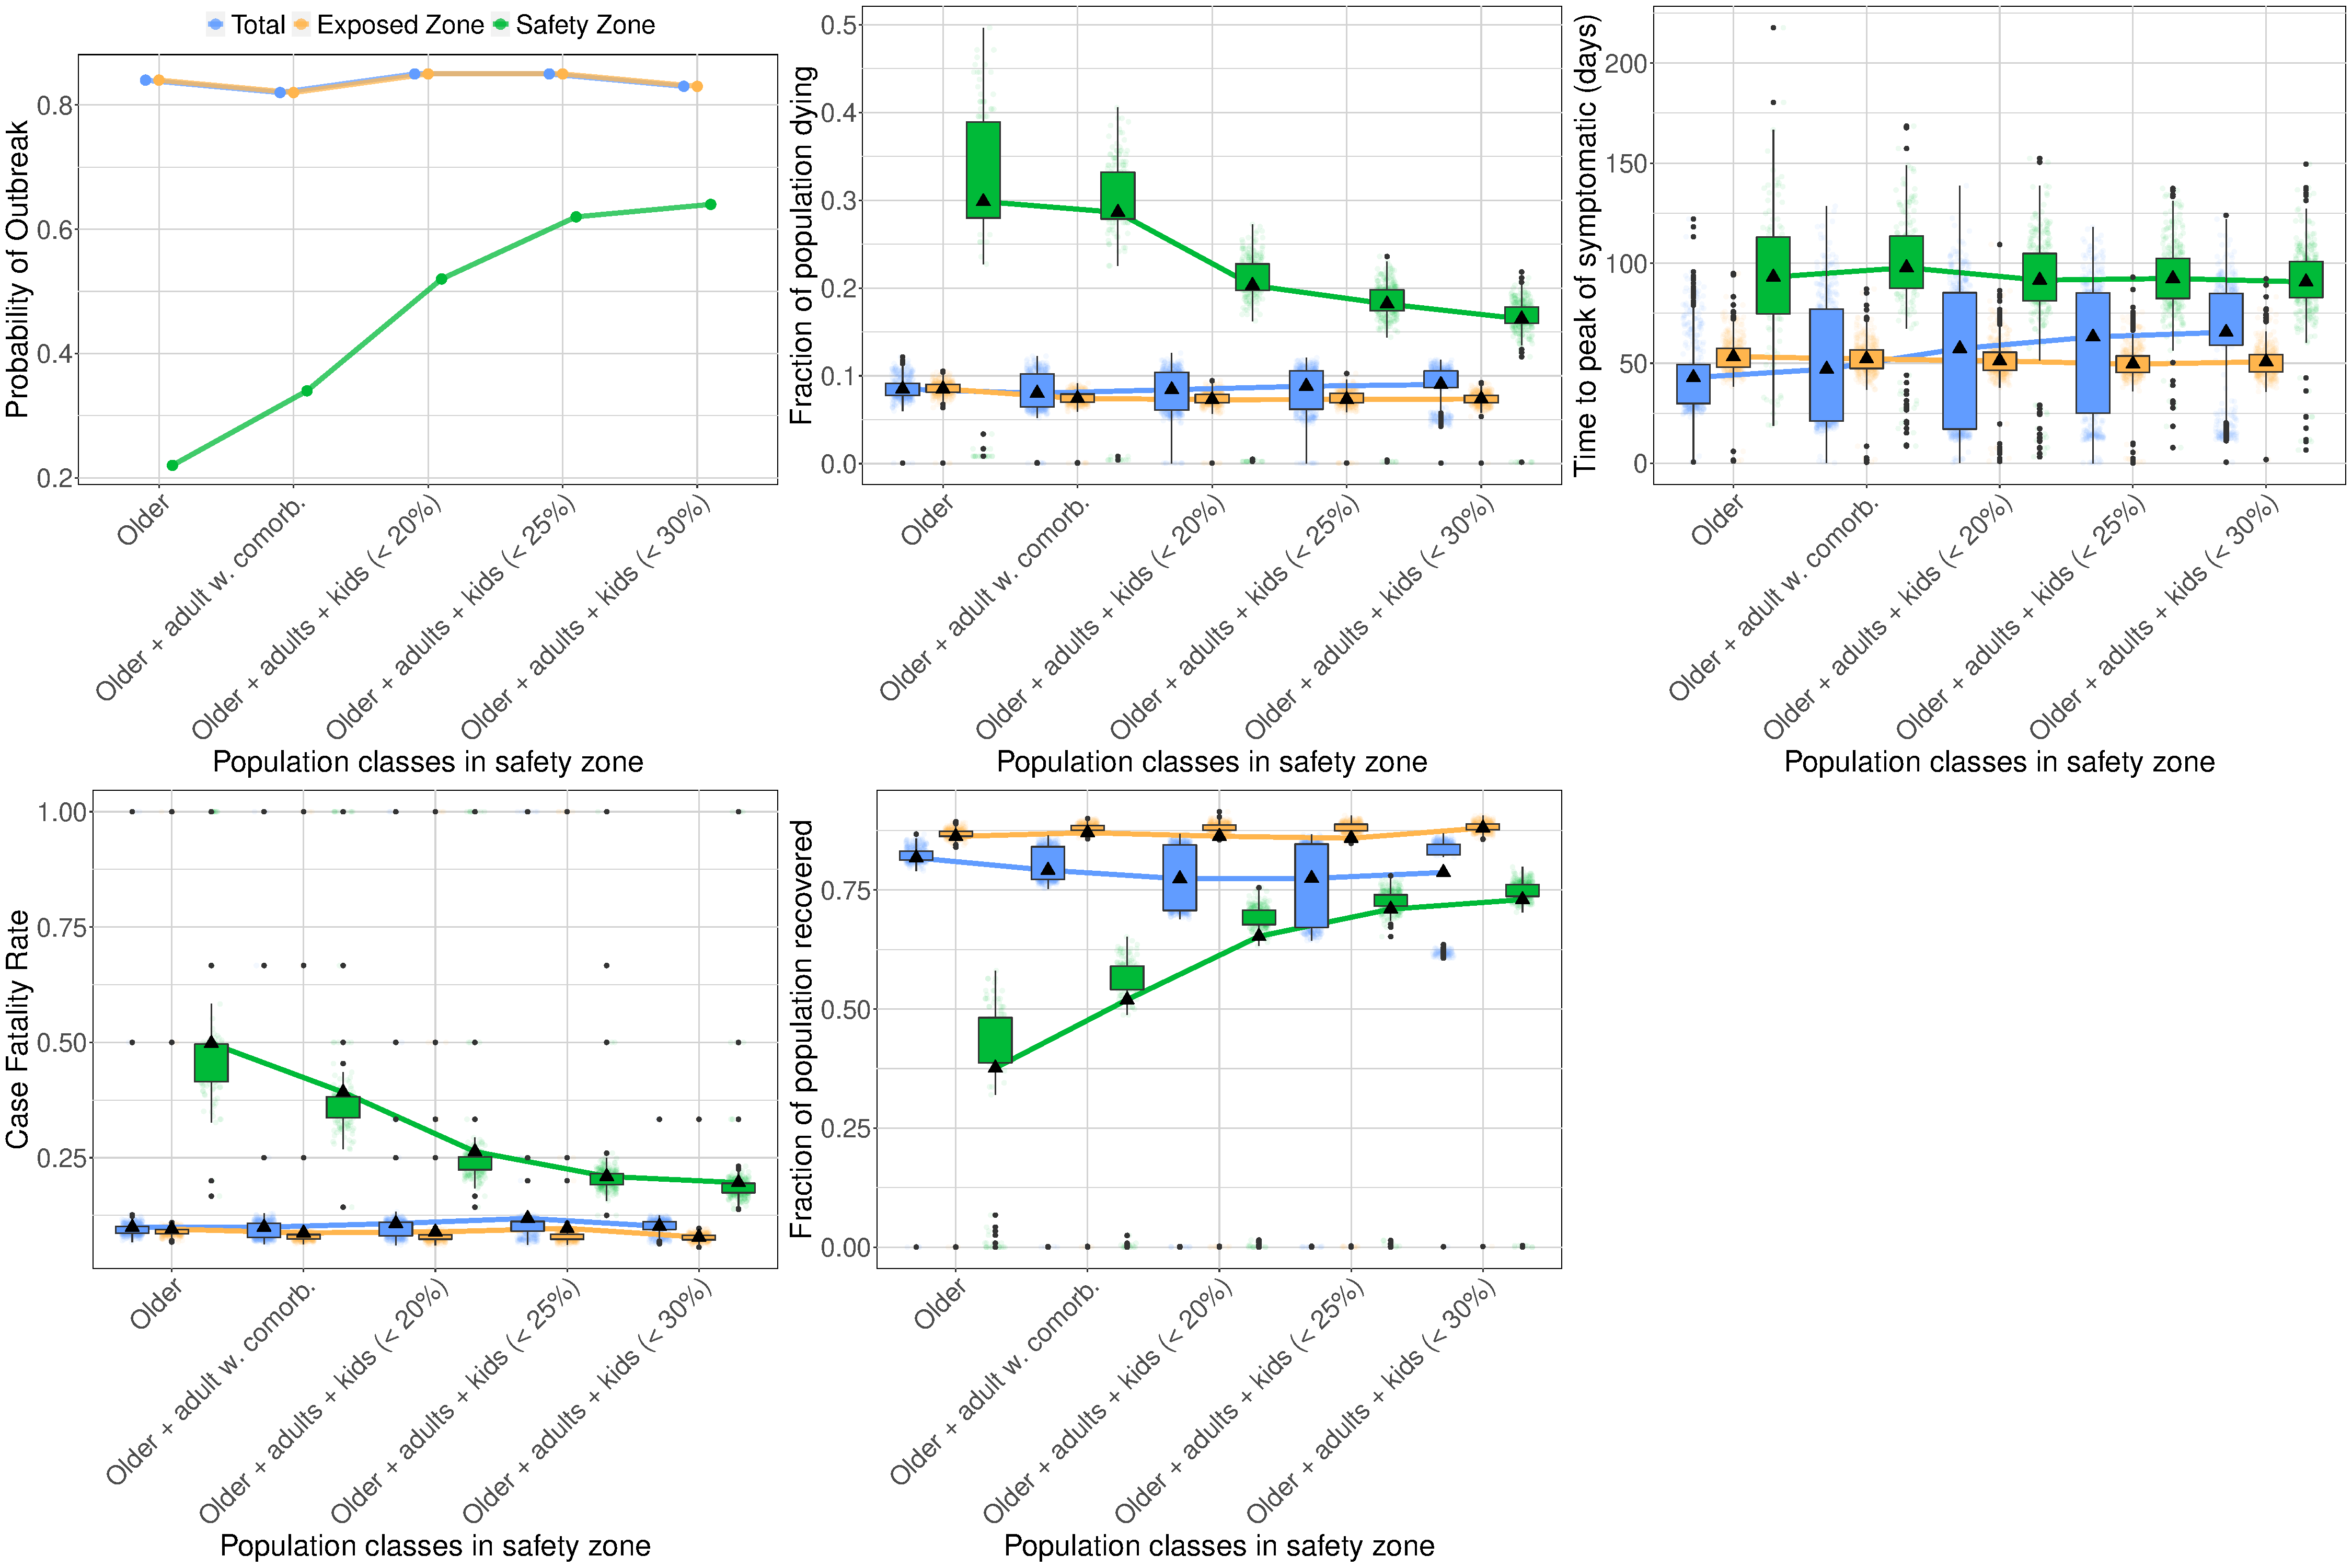
\includegraphics[width=1\textwidth]{figures/FigS9}\hspace{2mm}\caption{\label{fig:Suppl_safety} \textbf{Number of contacts in the buffer
zone.} IFR (left), and fraction of the population that recovers (right)
as a function of the number of contacts that each individual in the
safety zone has in the buffer zone per week. All figures consider
the scenario in which 20\% of the camp's population is allocated to
the safety zone.}
\end{figure}
\medskip{}

\begin{figure}[H]
\begin{centering}
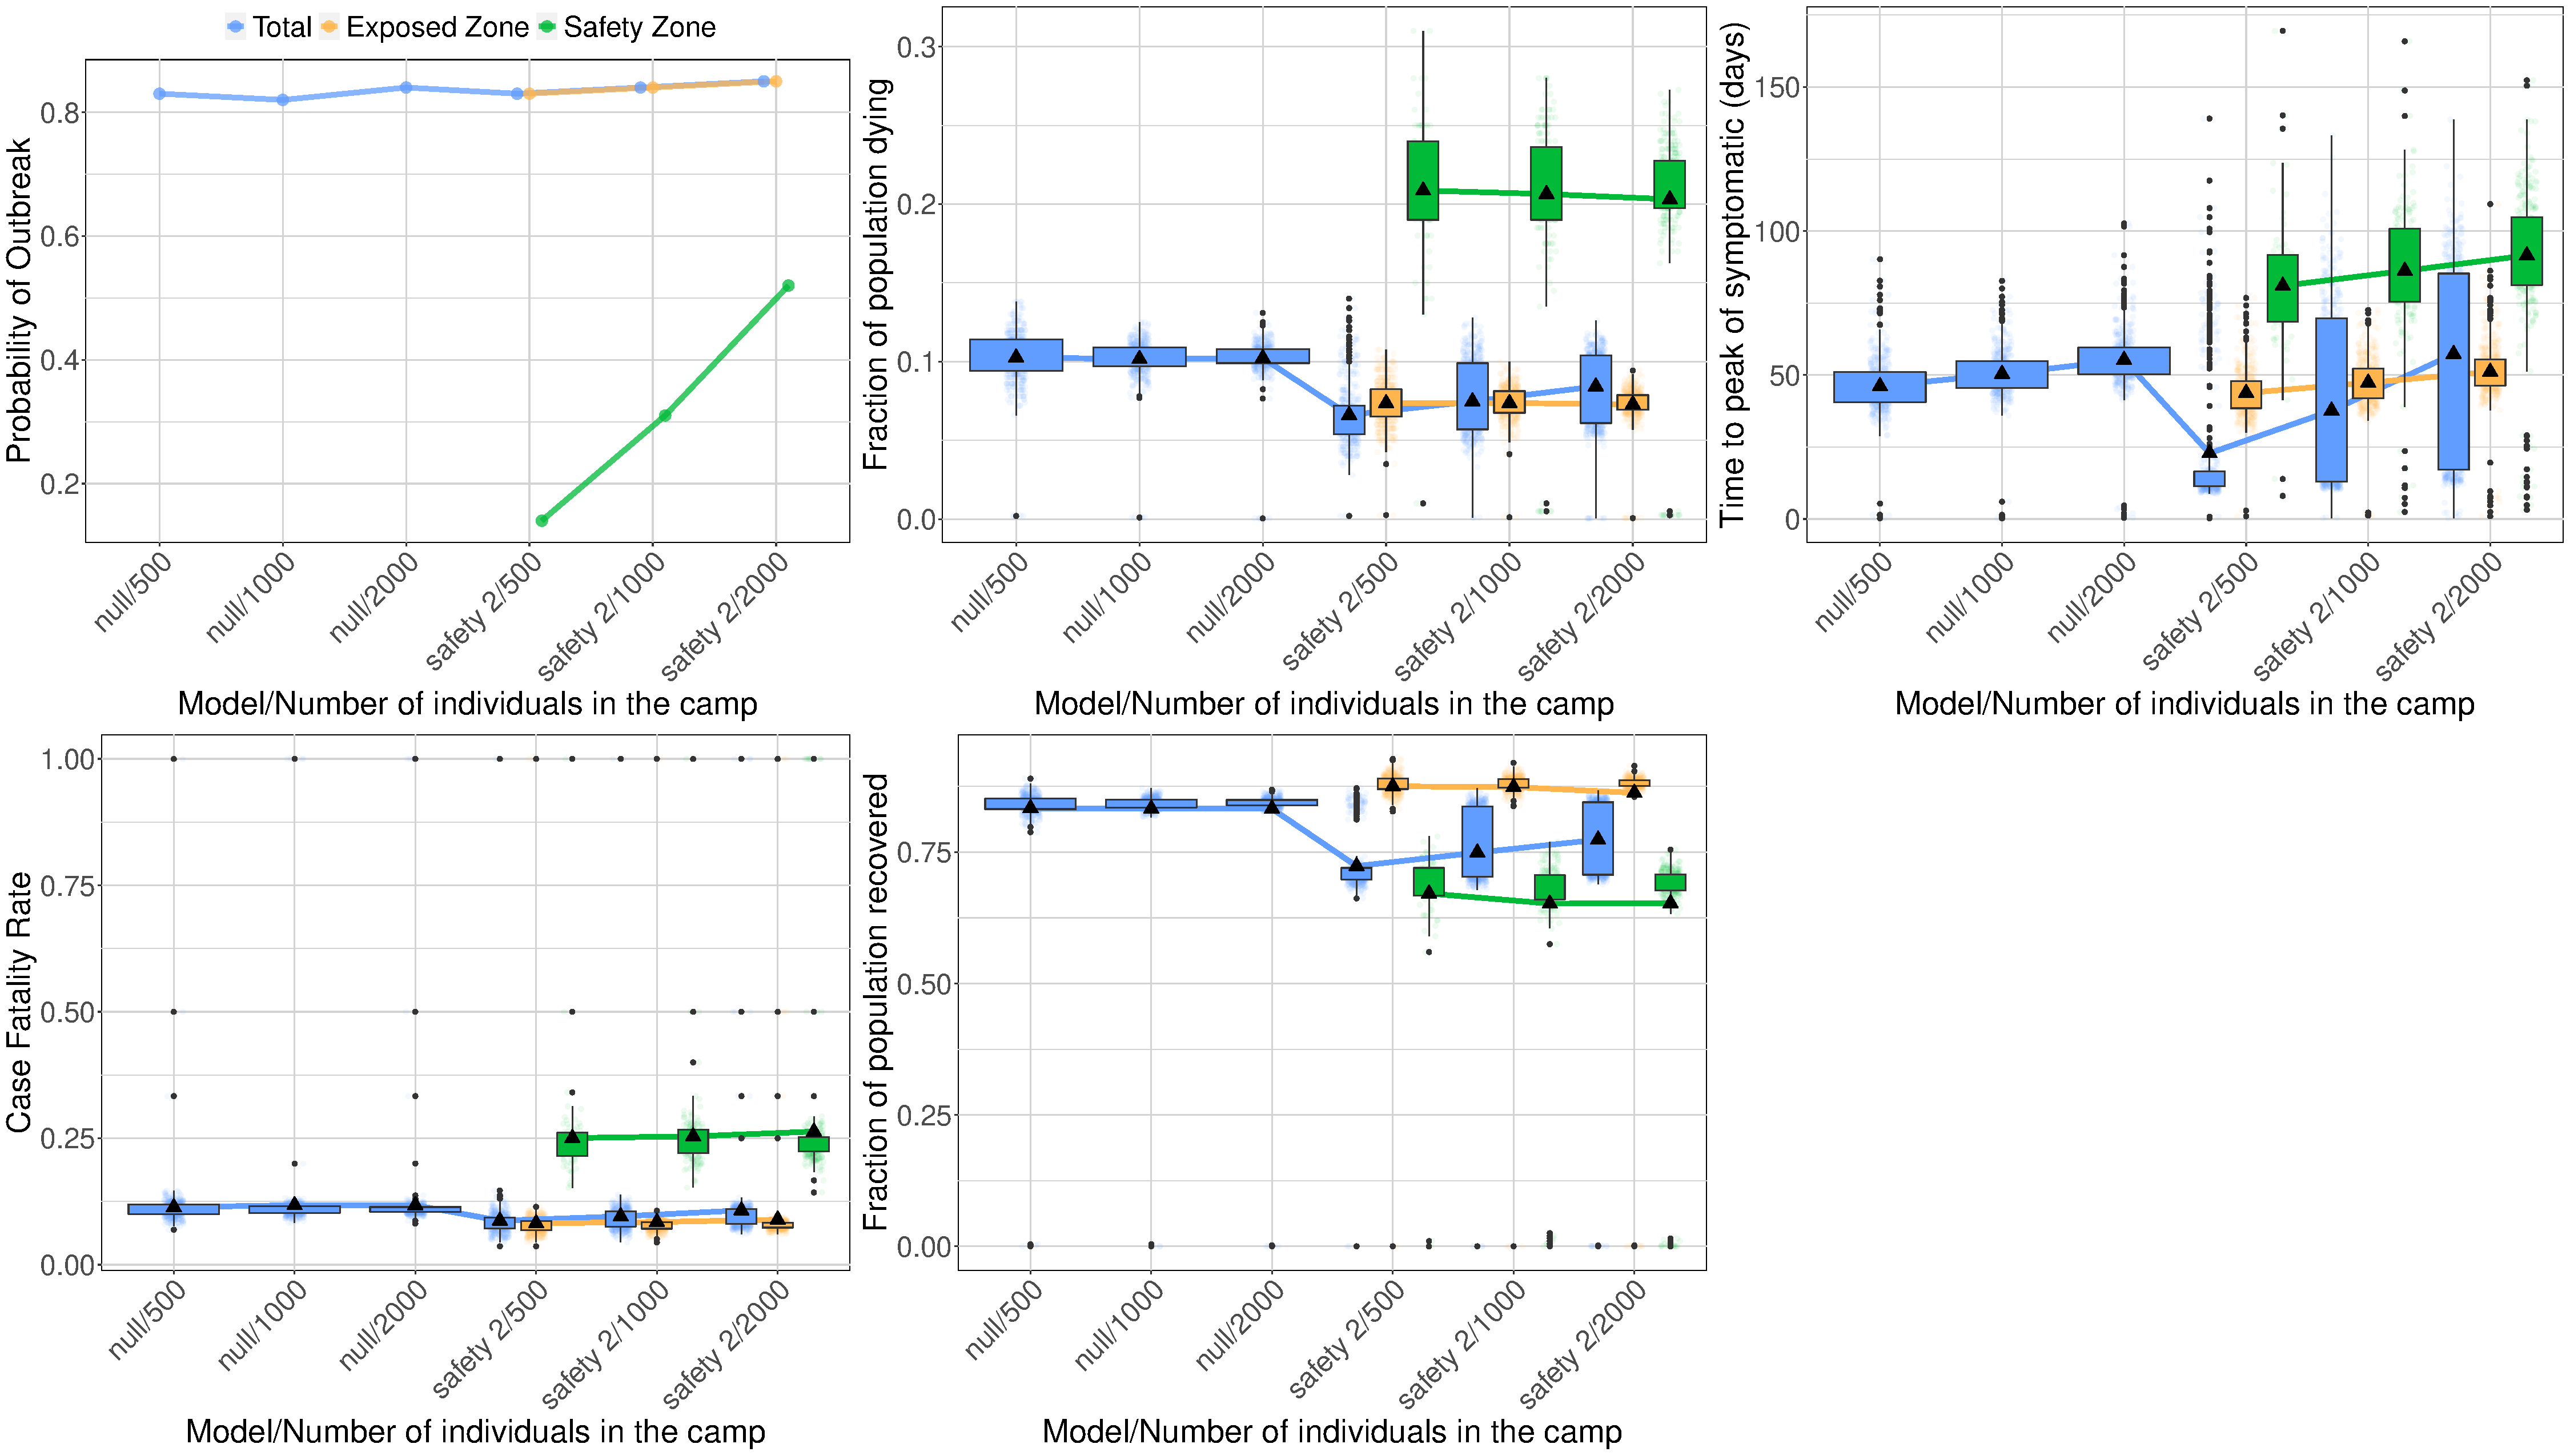
\includegraphics[width=1\textwidth]{figures/FigS10}\hspace{2mm}
\par\end{centering}
\caption{\label{fig:Suppl_popClass} \textbf{Population moving to the safety
zone.} Probability of an outbreak (top left), fraction of the population
dying (top middle), time until peak symptomatic cases (top right),
IFR (bottom left), and fraction of the population that recovers (bottom
middle) as a function of the safety zone allocation scenario (see
Table \ref{tab:SafetyScenarios}). All figures consider the scenario
with 2 contacts in the buffer per person in the safety zone per week.}
\end{figure}
\medskip{}

\begin{figure}[H]
\begin{centering}
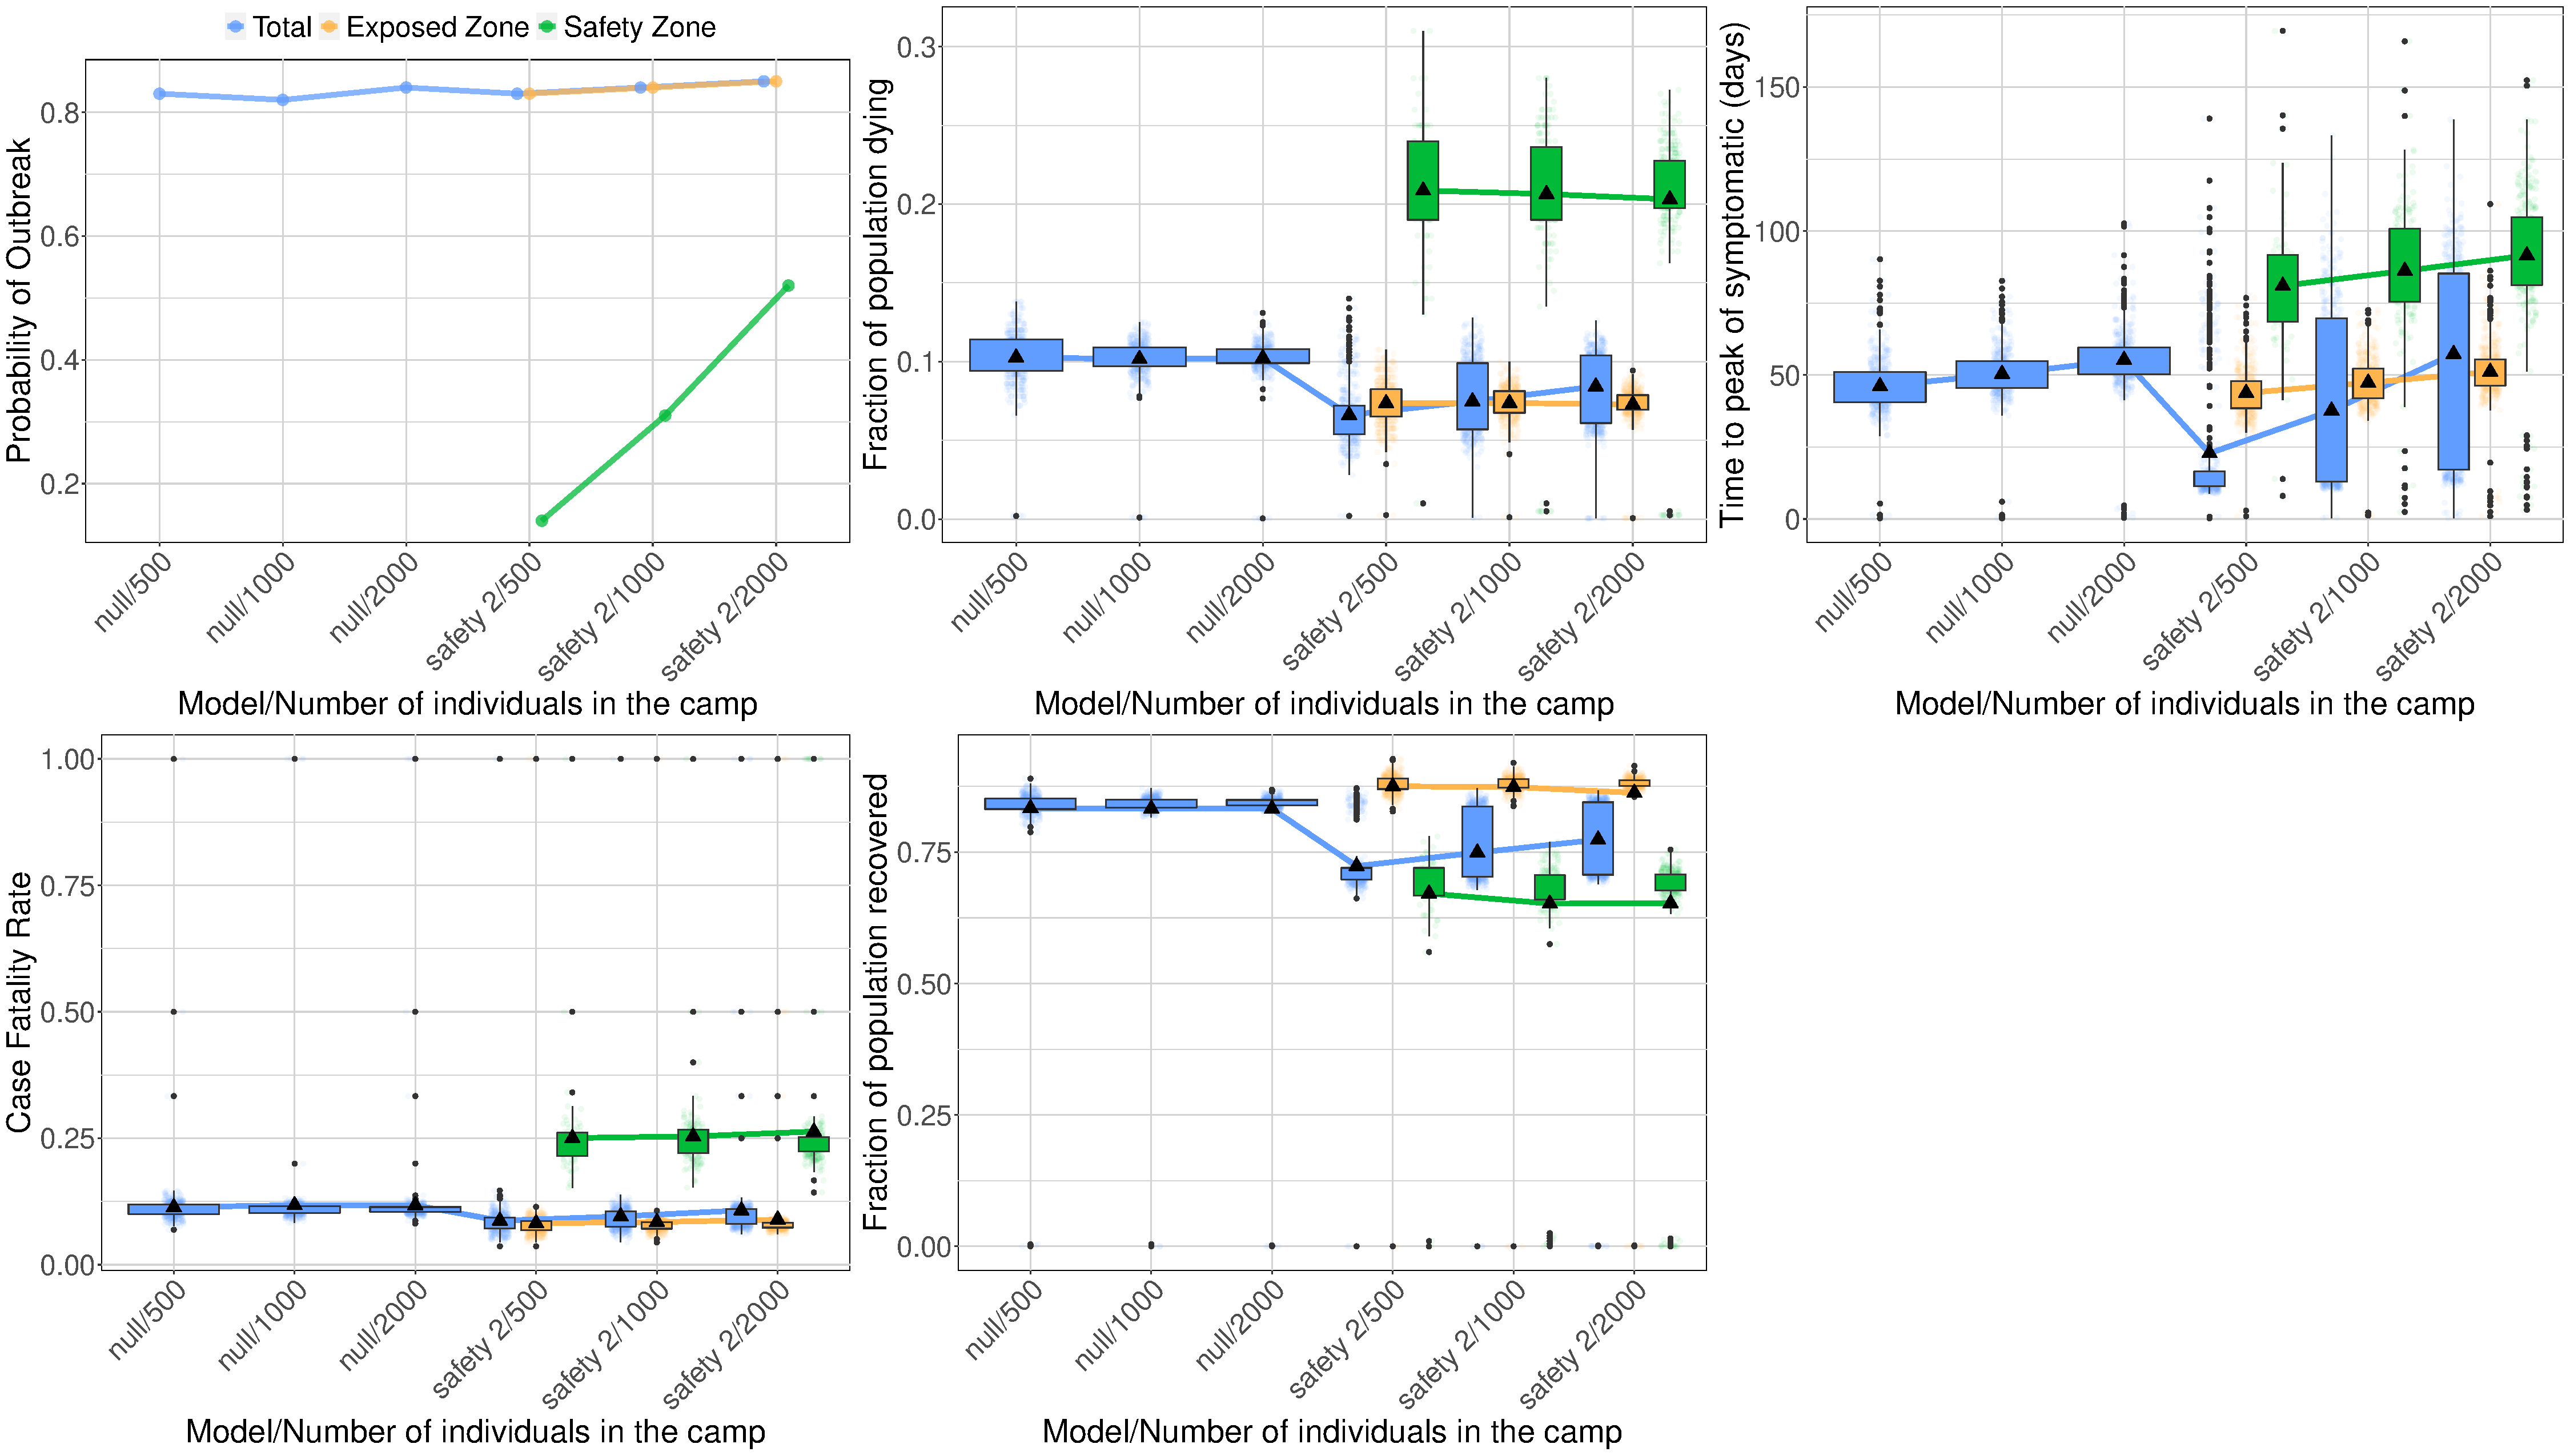
\includegraphics[width=1\textwidth]{figures/FigS11}\hspace{2mm}
\par\end{centering}
\caption{\label{fig:Suppl_popSize} \textbf{Efficacy of the safety zone for
different population sizes.} Probability of an outbreak (top left),
fraction of the population dying (top middle), time until peak symptomatic
cases (top right), IFR (bottom left), and fraction of the population
that recovers (bottom middle) as a function of the total population
size. The figures consider scenarios with no interventions (null),
and with a safety zone comprising 20\% of the camp's population with
2 contacts in the buffer zone per person in the safety zone per week
(safety 2).}
\end{figure}

\medskip{}

\begin{figure}[H]
\begin{centering}
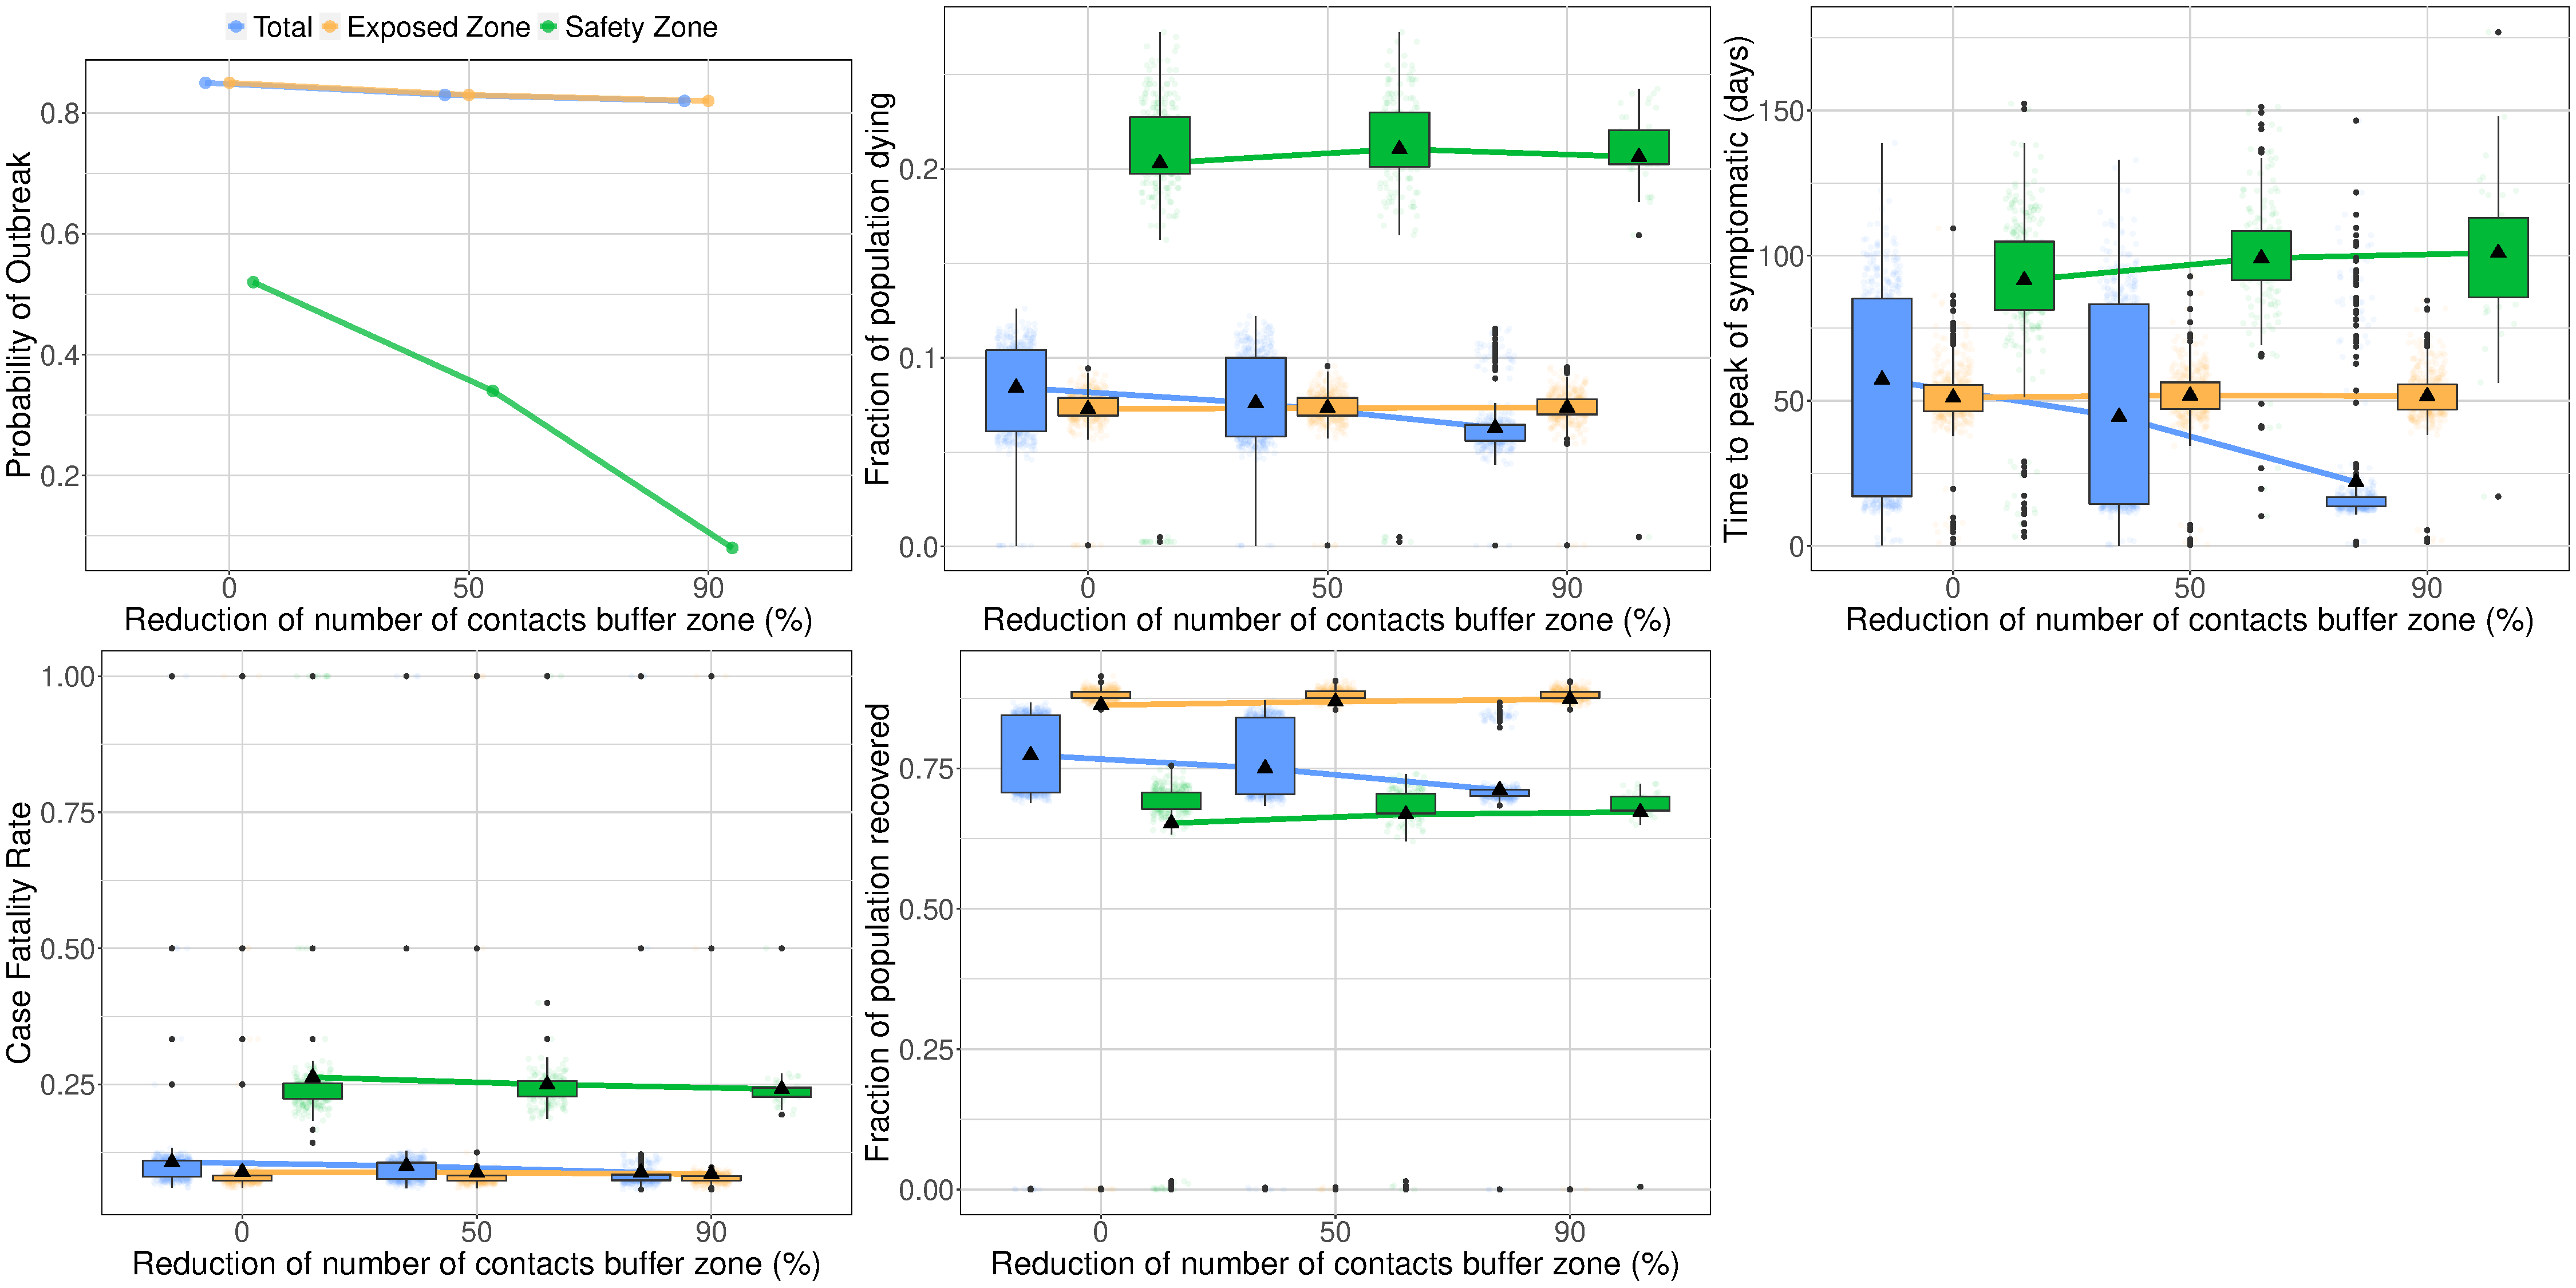
\includegraphics[width=1\textwidth]{figures/FigS12}\hspace{2mm}
\par\end{centering}
\caption{\label{fig:Suppl_lockdown} \textbf{Lockdown of the safety zone.}
Probability of an outbreak (top left), fraction of the population
dying (top middle), time until peak symptomatic cases (top right),
IFR (bottom left), and fraction of the population that recovers (bottom
middle) as a function of the reduction in the number of contacts permitted
in the buffer zone from a baseline of 2 per person in the safety zone
per week. All figures consider the scenario in which 20\% of the camp's
population is allocated to the safety zone.}
\end{figure}

\medskip{}

\begin{figure}[H]
\centering{}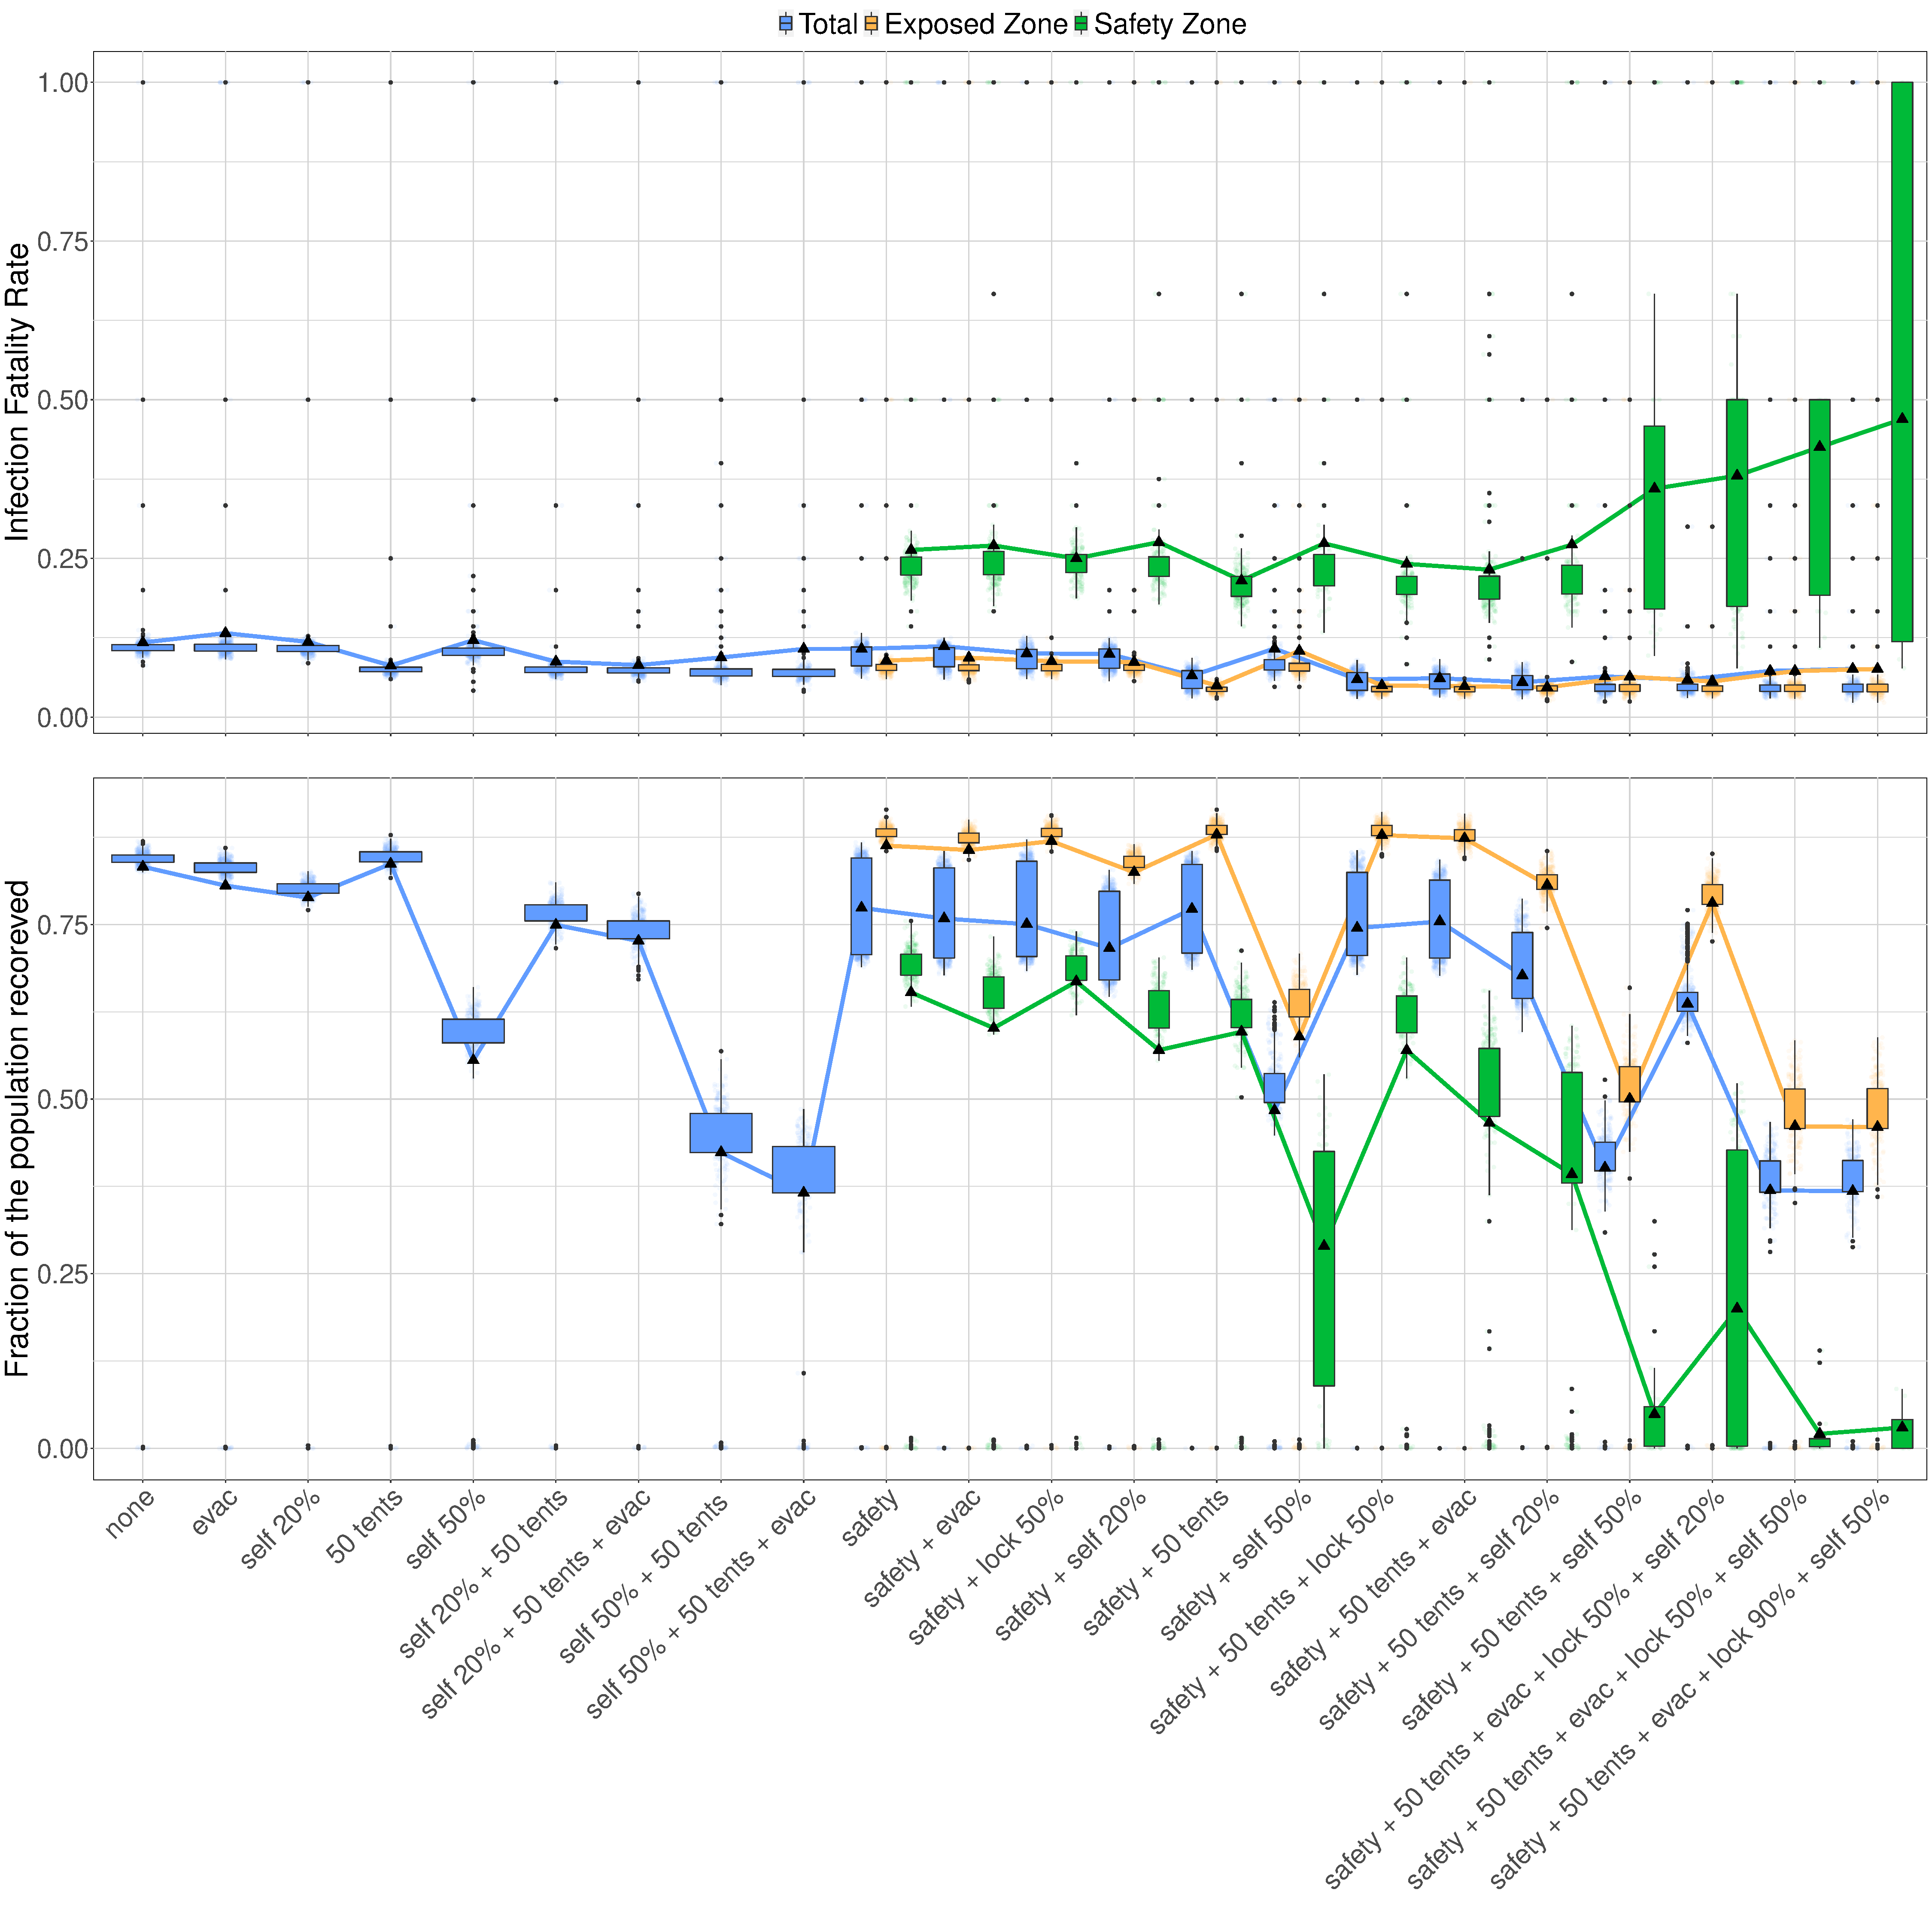
\includegraphics[height=0.7\textheight]{figures/FigS13}\hspace{2mm}\caption{\label{fig:Suppl_combined} \textbf{Combined interventions.} IFR (top),
and fraction of the population that recovers (bottom) for different
combinations of interventions. Evac = evacuation of severely symptomatic,
self = self-distancing, tents = number of available self-isolation
tents, safety = safety zone, lock = lockdown of the buffer zone. For
combinations of interventions including a safety zone, we distinguish
between the population living in the green zone, in the orange zone
and the whole population. The increase in the IFR for the green zone
is explained by the discretization of the possible values that the
IFR can take when the number of cases is very low (see Supplementary
Table \ref{tab:CFR_discrete}).}
\end{figure}

\begin{table}[H]
\begin{centering}
\includegraphics{figures/Table_S4}
\par\end{centering}
\caption{\label{tab:CFR_discrete} \textbf{Efficacy of the safety zone in combination
with other interventions.} \textless 20 cases = number of outbreaks
in the green zone with fewer than 20 cases recorded. Total = total
number of simulations where an outbreak in the green zone occurs (at
least one death). \% of total = percent of outbreaks where fewer than
20 cases are recorded. N = 500 simulations for each combination of
interventions. For the most effective combinations, the majority of
simulations where an outbreak occurs in the green zone see fewer than
20 cases. In these simulations, the discretization of the possible
values that the IFR can take explains its apparently anomalous increase
in Fig. \ref{fig:Suppl_combined}.}
\end{table}

\newpage{}

\bibliographystyle{unsrt}
\bibliography{req550-syria}

\end{document}
